% This is "sig-alternate.tex" V2.1 April 2013
% This file should be compiled with V2.5 of "sig-alternate.cls" May 2012
%
% This example file demonstrates the use of the 'sig-alternate.cls'
% V2.5 LaTeX2e document class file. It is for those submitting
% articles to ACM Conference Proceedings WHO DO NOT WISH TO
% STRICTLY ADHERE TO THE SIGS (PUBS-BOARD-ENDORSED) STYLE.
% The 'sig-alternate.cls' file will produce a similar-looking,
% albeit, 'tighter' paper resulting in, invariably, fewer pages.
%
% ----------------------------------------------------------------------------------------------------------------
% This .tex file (and associated .cls V2.5) produces:
%       1) The Permission Statement
%       2) The Conference (location) Info information
%       3) The Copyright Line with ACM data
%       4) NO page numbers
%
% as against the acm_proc_article-sp.cls file which
% DOES NOT produce 1) thru' 3) above.
%
% Using 'sig-alternate.cls' you have control, however, from within
% the source .tex file, over both the CopyrightYear
% (defaulted to 200X) and the ACM Copyright Data
% (defaulted to X-XXXXX-XX-X/XX/XX).
% e.g.
% \CopyrightYear{2007} will cause 2007 to appear in the copyright line.
% \crdata{0-12345-67-8/90/12} will cause 0-12345-67-8/90/12 to appear in the copyright line.
%
% ---------------------------------------------------------------------------------------------------------------
% This .tex source is an example which *does* use
% the .bib file (from which the .bbl file % is produced).
% REMEMBER HOWEVER: After having produced the .bbl file,
% and prior to final submission, you *NEED* to 'insert'
% your .bbl file into your source .tex file so as to provide
% ONE 'self-contained' source file.
%
% ================= IF YOU HAVE QUESTIONS =======================
% Questions regarding the SIGS styles, SIGS policies and
% procedures, Conferences etc. should be sent to
% Adrienne Griscti (griscti@acm.org)
%
% Technical questions _only_ to
% Gerald Murray (murray@hq.acm.org)
% ===============================================================
%
% For tracking purposes - this is V2.0 - May 2012
\documentclass[sigconf,authordraft]{acmart}
              \usepackage{booktabs,enumitem}\acmConference[VAM-HRI'18]{1st
                International Workshop on Virtual, Augmented, and
                Mixed Reality for Human-Robot Interaction}{March 2018}{Chicago, Illinois, USA} \acmYear{2018}
%\documentclass{sig-alternate-05-2015}
\usepackage{graphicx,caption}
%\usepackage{hyperref}
\usepackage{url}
\let\labelindent\relax
\usepackage[keeplastbox]{flushend}
\usepackage{amsmath,amssymb,enumitem}
\usepackage{xcolor}\newcommand\todo[1]{\textcolor{blue}{#1}}
\begin{document}

%% % Copyright
%% \setcopyright{acmcopyright}
%% %\setcopyright{acmlicensed}
%% %\setcopyright{rightsretained}
%% %\setcopyright{usgov}
%% %\setcopyright{usgovmixed}
%% %\setcopyright{cagov}
%% %\setcopyright{cagovmixed}


%% % DOI
%% \doi{10.475/123_4}

%% % ISBN
%% \isbn{123-4567-24-567/08/06}

%% %Conference
%% %\conferenceinfo{PLDI '13}{June 16--19, 2013, Seattle, WA, USA}

%% \acmPrice{\$15.00}

%
% --- Author Metadata here ---
%\conferenceinfo{HRI}{2017 Vienna, Austria}
%\CopyrightYear{2007} % Allows default copyright year (20XX) to be over-ridden - IF NEED BE.
%\crdata{0-12345-67-8/90/01}  % Allows default copyright data (0-89791-88-6/97/05) to be over-ridden - IF NEED BE.
% --- End of Author Metadata ---

%\title[Interaction with Teleoperated and Autonomous Humanoids]{Differences in Interaction Patterns and Perception\\ for Teleoperated and Autonomous Humanoid Robots}


\title{Investigating Interactions with Teleoperated and Autonomous Humanoids Using a Suit-Based VR Teleoperation Interface}

%
% You need the command \numberofauthors to handle the 'placement
% and alignment' of the authors beneath the title.
%
% For aesthetic reasons, we recommend 'three authors at a time'
% i.e. three 'name/affiliation blocks' be placed beneath the title.
%
% NOTE: You are NOT restricted in how many 'rows' of
% "name/affiliations" may appear. We just ask that you restrict
% the number of 'columns' to three.
%
% Because of the available 'opening page real-estate'
% we ask you to refrain from putting more than six authors
% (two rows with three columns) beneath the article title.
% More than six makes the first-page appear very cluttered indeed.
%
% Use the \alignauthor commands to handle the names
% and affiliations for an 'aesthetic maximum' of six authors.
% Add names, affiliations, addresses for
% the seventh etc. author(s) as the argument for the
% \additionalauthors command.
% These 'additional authors' will be output/set for you
% without further effort on your part as the last section in
% the body of your article BEFORE References or any Appendices.

%\numberofauthors{3} %  in this sample file, there are a *total*
% of EIGHT authors. SIX appear on the 'first-page' (for formatting
% reasons) and the remaining two appear in the \additionalauthors section.
%
  % You can go ahead and credit any number of authors here,
  % e.g. one 'row of three' or two rows (consisting of one row of three
  % and a second row of one, two or three).
  %
  % The command \alignauthor (no curly braces needed) should
  % precede each author name, affiliation/snail-mail address and
  % e-mail address. Additionally, tag each line of
  % affiliation/address with \affaddr, and tag the
  % e-mail address with \email.
  %
  % 1st. author
\author{Maxwell Bennett}
\affiliation{\institution{Kindred}\streetaddress{169 Stillman St.}\city{San Francisco}\state{California}\postcode{94110}}
\email{maxwellbbennett@gmail.com}
\author{Tom Williams}
\affiliation{\institution{MIRRORLab\\Colorado School of
    Mines}\streetaddress{1500 Illinois
    St.}\city{Golden}\state{CO}\postcode{80202}}
\email{twilliams@mines.edu}
\author{Daria Thames}
\affiliation{\institution{HRILab\\Tufts University}\streetaddress{200
    Boston Ave.}\city{Medford}\state{MA}\postcode{02155}}
\email{daria.thames@tufts.edu}
\author{Matthias Scheutz}
\affiliation{\institution{HRILab\\Tufts University}\streetaddress{200
    Boston Ave.}\city{Medford}\state{MA}\postcode{02155}}
\email{matthias.scheutz@tufts.edu}
 
  % 2nd. author
  %% \alignauthor
  %% G.K.M. Tobin\titlenote{The secretary disavows
  %% any knowledge of this author's actions.}\\
  %%        \affaddr{Institute for Clarity in Documentation}\\
  %%        \affaddr{P.O. Box 1212}\\
  %%        \affaddr{Dublin, Ohio 43017-6221}\\
  %%        \email{webmaster@marysville-ohio.com}
  %% % 3rd. author
  %% \alignauthor Lars Th{\o}rv{\"a}ld\titlenote{This author is the
  %% one who did all the really hard work.}\\
  %%        \affaddr{The Th{\o}rv{\"a}ld Group}\\
  %%        \affaddr{1 Th{\o}rv{\"a}ld Circle}\\
  %%        \affaddr{Hekla, Iceland}\\
  %%        \email{larst@affiliation.org}
  %% \and  % use '\and' if you need 'another row' of author names
  %% % 4th. author
  %% \alignauthor Lawrence P. Leipuner\\
  %%        \affaddr{Brookhaven Laboratories}\\
  %%        \affaddr{Brookhaven National Lab}\\
  %%        \affaddr{P.O. Box 5000}\\
  %%        \email{lleipuner@researchlabs.org}
  %% % 5th. author
  %% \alignauthor Sean Fogarty\\
  %%        \affaddr{NASA Ames Research Center}\\
  %%        \affaddr{Moffett Field}\\
  %%        \affaddr{California 94035}\\
  %%        \email{fogartys@amesres.org}
  %% % 6th. author
  %% \alignauthor Charles Palmer\\
  %%        \affaddr{Palmer Research Laboratories}\\
  %%        \affaddr{8600 Datapoint Drive}\\
  %%        \affaddr{San Antonio, Te
  %%   xas 78229}\\
       %% \email{cpalmer@prl.com}
%}
% There's nothing stopping you putting the seventh, eighth, etc.
% author on the opening page (as the 'third row') but we ask,
% for aesthetic reasons that you place these 'additional authors'
% in the \additional authors block, viz.
%% \additionalauthors{Additional authors: John Smith (The Th{\o}rv{\"a}ld Group,
%% email: {\texttt{jsmith@affiliation.org}}) and Julius P.~Kumquat
%% (The Kumquat Consortium, email: {\texttt{jpkumquat@consortium.net}}).}
%% \date{30 July 1999}
% Just remember to make sure that the TOTAL number of authors
% is the number that will appear on the first page PLUS the
% number that will appear in the \additionalauthors section.

%\thispagestyle{empty}
%\pagestyle{empty}

\begin{abstract}  
With the increased use of teleoperated humanoid robots, it is
important to understand how physical embodiment and perceived autonomy
affect how humans instruct autonomous and teleoperated robots, as well
as humans.
%% it is important to recognize whether any differences between instructions
%% given to humans and to robots are due to the physical embodiment or 
%% to the perceived autonomy of the instructee.
%% As sliding autonomy and shared control are increasingly used in
%% teleoperated and telepresence robots, it becomes increasingly
%% important to understand how differing levels 
%% of robot autonomy affect how humans interact with such
%% robots.
In this paper, we discuss how a novel suit-based VR teleoperation
interface and paired humanoid robot allowed us to investigate these
differences. We present both our empirical results, as well as lessons
learned with respect to the design and use of such teleoperation interfaces.

%% Our results suggest that humans will use politeness
%% strategies equally with human, autonomous robotic, and
%% teleoperated robotic teammates, reinforcing
%% recent findings that autonomous robots must % be able to
%% comprehend and appropriately respond to human utterances that follow
%% such strategies.
%% %
%% Our results also suggest variations in how %these
%%  different
%% teammates were perceived. Specifically, our results suggest that human-teleoperated robots were perceived as less intelligent than human
%% teammates; a finding 
%% with serious implications for human-robot team dynamics.
\end{abstract}


%
% The code below should be generated by the tool at
% http://dl.acm.org/ccs.cfm
% Please copy and paste the code instead of the example below. 
%
%\begin{CCSXML}
%<ccs2012>
% <concept>
%  <concept_id>10010520.10010553.10010562</concept_id>
%  <concept_desc>Computer systems organization~Embedded systems</concept_desc>
%  <concept_significance>500</concept_significance>
% </concept>
% <concept>
%  <concept_id>10010520.10010575.10010755</concept_id>
%  <concept_desc>Computer systems organization~Redundancy</concept_desc>
%  <concept_significance>300</concept_significance>
% </concept>
% <concept>
%  <concept_id>10010520.10010553.10010554</concept_id>
%  <concept_desc>Computer systems organization~Robotics</concept_desc>
%  <concept_significance>100</concept_significance>
% </concept>
% <concept>
%  <concept_id>10003033.10003083.10003095</concept_id>
%  <concept_desc>Networks~Network reliability</concept_desc>
%  <concept_significance>100</concept_significance>
% </concept>
%</ccs2012>  
%\end{CCSXML}

%\ccsdesc[500]{Computer systems organization~Embedded systems}
%\ccsdesc[300]{Computer systems organization~Redundancy}
%\ccsdesc{Computer systems organization~Robotics}
%\ccsdesc[100]{Networks~Network reliability}


%
% End generated code
%

%
%  Use this command to print the description
%
%\printccsdesc

% We no longer use \terms command
%\terms{Theory}

%\keywords{Teleoperation; telepresence; autonomy; humanoid robots, user
%studies}
\maketitle


\section{Introduction}
%% \todo{Why does this start re: physical capabilities, while the
%%   abstract starts re: linguistic capabilities?}
It is becoming increasingly important to understand how
humans will perceive and instruct robots. Knowing
how humans will instruct robots is especially important both for
robot developers seeking to enable learning-from-demonstration capabilities
as well as those seeking to work with robots in more collaborative
tasks requiring sophisticated motion or dexterity.


What is more, with the increased use of teleoperated humanoid robots,
it is important to recognize whether any such differences are due to
the physical embodiment or to the perceived level of autonomy of the instructee.
While some previous
work~\cite{schreitter2014exploring,SCHREITTER16.343} has begun to look
at linguistic 
differences in human-to-human and human-to-robot instructions, it has
not considered such possible effects. Furthermore, in that work a
specific instruction task was provided by the experimenters, which may
have biased the utterances used in 
task instructions.
%
%% Thus, in this paper we present an experiment
%% investigating the linguistic differences between human-to-human and
%% human-to-robot task instructions %for both autonomous and teleoperated
%% %robots 
%% using a paradigm in which participants sequentially teach a human and
%% a robot (believed by participants to be either autonomous or
%% human-teleoperated) how to arrange a set of objects in a unique manner
%% and determined by each participant. 
%
%To better understand the causes of linguistic differences, %% whether any differences were due to
%%% perceived differences in either physical embodiment or autonomy,
%we also evaluated
%the differences between participants' perceptions of autonomous versus
%teleoperated humanoid robots. 
Little empirical research in HRI has investigated
perceptions of teleoperated humanoid robots, and to the best of our
knowledge all previous research investigating human perceptions of
autonomous versus teleoperated robots has been \textit{observational},
in addition to using robots controlled
through graphical interfaces.

In this paper we describe a novel VR teleoperation interface
in which teleoperator motions are replicated by a
robot in real time, and
discuss how it allowed us to better investigate \emph{interaction} differences between
human-to-human and human-to-robot task instructions, as originally
described in our previous work~\cite{bennett2017differences}.

%% , allowing realistic, spontaneous, task-based
%% interactions.

%% As sliding autonomy and shared control are increasingly used in
%% teleoperated and telepresence robots, it becomes increasingly
%% important to understand how differing levels 
%% of robot autonomy affect how humans interact with such
%% robots.

%% In Section~\ref{sec:rw} we discuss previous work informing
%% our experiment.
%% %% describe the novel dimensions
%% %% of this experiment through a deeper analysis of previous work.
%% In
%% Section~\ref{sec:exp} we then discuss the design
%% of a human-subject experiment to investigate our questions of
%% interest. In Section~\ref{sec:results} we present the results of that
%% experiment, and discuss our findings in
%% Section~\ref{sec:disc}. Finally, we conclude with design
%% recommendations and directions for future work in Section~\ref{sec:conc}.

%% =======================================================================

%% In this paper, we present the results of a human-subject
%% experiment in which participants interacted with both a human and a
%% suit-based teleoperated humanoid robot said to be either autonomous
%% or teleoperated, in a collaborative, task-based
%% setting. 

%% Our results suggest that humans will use politeness
%% strategies with human teammates, autonomous robot teammates, and
%% teleoperated robot teammates, at an equivalent rate, reinforcing
%% recent findings that autonomous robots must be able to
%% comprehend and appropriately respond to human utterances that follow
%% such strategies.
%% %
%% Our results also suggest differences in how these three types of
%% teammates were perceived. Specifically, we found
%% differences in perceived intelligence and credit assignment between
%% human, teleoperated robot, and autonomous robot teammates; a finding
%% with serious implications for human-robot team dynamics.

%% =======================================================================

%% Recent advances in robotic, virtual reality, and mobile technologies
%% have produced new opportunities for users to observe and engage with
%% remote environments through telepresence and teleoperation
%% technologies~\cite{rae2015everyday}. These technologies are now being
%% regularly used in a variety of application domains, including in
%% business settings
%% (e.g., the Beam~\cite{Beam} and VGo~\cite{VGo} telepresence robots),
%% medical settings (e.g., the da Vinci surgical robot~\cite{Vinci}), and
%% the home (e.g. 
%% %soon-to-ship 
%% Jibo~\cite{Jibo}).

%% Simultaneously, there has been increased interest in allowing such
%% systems to employ sliding autonomy or shared control, in which a human
%% teleoperator might temporarily release control in order to allow
%% autonomous completion of specific behaviors and
%% actions~\cite{crandall2002characterizing,coltin2011effective}. Such
%% control schemes may allow the teleoperator to avoid procedures that
%% are highly effortful yet easily automated (e.g., targeted
%% grasping~\cite{leeper2012strategies}), or may allow the 
%% teleoperator to simultaneously teleoperate multiple robots~\cite{heger2006sliding}. 
%% Alternatively, sliding autonomy or shared control can be valuable in situations
%% in which a robot behaves autonomously by default, but needs to be
%% teleoperated in order to perform specific tasks that are particularly
%% complex~\cite{mast2015semi} or ethically fraught~\cite{sparrow2009building}.


%% As sliding autonomy and shared control are increasingly used in
%% teleoperated and telepresence robots, it becomes increasingly
%% important to understand how differing levels 
%% of robot autonomy affect how humans interact with such
%% robots. Intuitively, we would expect people to perceive and interact
%% with teleoperated robots in substantially different
%% ways than they interact with completely autonomous robots or with
%% fully present human teammates. There are clear differences between how
%% humans perceive and interact with robots with respect to other humans;
%% it is unclear where along this spectrum of perception and
%% interaction teleoperated robots will fall. 

%% This is a question that has been of interest to a number of
%% researchers in recent years~\cite{rae2015everyday}, but the majority of this research has
%% fallen behind the state of the art in teleoperation. For several
%% decades, there has been continual progress on teleoperated
%% \textit{humanoid} robots~\cite{goodrich2013teleoperation}; but, with
%% the exception of a few notable examples
%% (e.g. ~\cite{weiss2009autonomous}), most empirical research into human
%% interaction with teleoperated robots has not made use of teleoperated
%% humanoid robots. Humanoid robots are uniquely suited to perform many
%% tasks a human might wish to perform in a remote environment, and will
%% likely have an easier time navigating and interacting with
%% environments designed for human beings~\cite{goodrich2013teleoperation}.
%% But research has shown that the form factor of humanoid robots may
%% cause them to be perceived using the same cognitive processes normally
%% used specifically to perceive other human
%% agents~\cite{oztop2005human}; this makes it especially important for
%% studies of interaction with teleoperated robots to make use of
%% humanoid robots.

%% Furthermore, these questions are increasingly important for
%% researchers in areas in which 
%% differential interaction is expected or even desired. In 
%% robot-facilitated autism therapy, for example, robots are used
%% precisely because it is known that autistic children will perceive and
%% interact with robots differently than they would with human
%% therapists~\cite{goodrich2013teleoperation}. Investigating differences
%% in perception of teleoperated and autonomous robots may help clarify
%% the benefits and appropriate usage of different control methods in
%% such contexts. 

%% In addition, much of the previous interactional research with
%% teleoperated robots has used robots controlled using joysticks
%% or Graphical User Interfaces (GUIs) within a Wizard-of-Oz paradigm
%% ~\cite{Stilman2008humanoid, goodrich2013teleoperation}. For 
%% teleoperated humanoid robots, however, it is crucial that interaction
%% studies make use of teleoperation interfaces that replicate the
%% natural motions of human teleoperators, as this may greatly increase
%% the perceived human-likeness of the robot. Furthermore, if more
%% coarse-grained user interfaces (e.g., joysticks and GUIs) are used to
%% teleoperate humanoid robots in interaction studies, this inherently
%% limits the degree to which the robot's behaviors may be uniquely
%% tailored to participants' demands. 

%% Finally, while there has been some previous research into human
%% perception of teleoperated and autonomous humanoid robots, that
%% research has studied how humans view such robots in observational
%% videos~\cite{weiss2009autonomous}. Much evidence suggests that human
%% perceptions of robots in observation greatly differ from human
%% perceptions of robots when actually interacted
%% with~\cite{woods2006comparing,bainbridge2008effect,bainbridge2011benefits}. 

%% In this paper, we present new empirical findings regarding difference
%% in human perception of and interaction with robots that they believe
%% to be teleoperated versus those that they believe to be
%% autonomous. In order for our results to be maximally applicable to the
%% state-of-the art of teleoperated robotics, our study makes use of a
%% humanoid robot. Furthermore, we make use of a
%% novel, immersive teleoperation interface in which a teleoperators'
%% motions are replicated on the teleoperated robot in real time: this
%% both emphasizes the potential
%% human-likeness of teleoperated humanoid robots, and allows the
%% teleoperated robot to engage in realistic, spontaneous, task-based
%% interactions. 

%% The rest of this paper will proceed as follows: In
%% Section~\ref{sec:rw} we discuss related work on our questions of
%% interest in further depth. In Section~\ref{sec:exp} we discuss the design
%% of a human-subject experiment to investigate our questions of
%% interest. In Section~\ref{sec:results} we present the results of that
%% experiment, and discuss our findings in
%% Section~\ref{sec:disc}. Finally, we conclude with design
%% recommendations and directions for future work in Section~\ref{sec:conc}.

%% \textbf{these are the novel aspects of the research, should that be explicitly stated?}Thus, by using a third party's novel one-to-one teleoperation technology to conduct the present research, we allowed for a human operator to immersively teleoperate a humanoid robot in realistic task-based interactions that were not preplanned or scripted. Additionally, with the real time teleoperation, we were able to study the differences in how people actually interact with robots instead of studying how they observe robots or interactions (with videos or photos), and thus we can study how language patterns differ when interacting with autonomous vs. teleoperated agents.
  

%% \textbf{is there something more to say here about not having it embody a human face (e.g. like Beam, or a telecom'd face)? Or any mention of potential uncanny valley effect?}



%% In this paper, we investigate these research questions using an
%% empirical study in which participants engaged in a natural, task-based
%% interaction with a teleoperated humanoid robot. To facilitate this
%% investigation, we make use of the previously mentioned, third-party, one-to-one immersive telepresence technology in which a human controls a humanoid robot using an exo-skeleton for arm movements, virtual reality for immersive vision and head movement, and pedals for wheeled movement.

\section{Related Work}
\label{sec:rw}

%\subsection{Linguistic Interaction with Robots vs. Humans}
%Recently, there has been much %% a significant amount
%%% of
%research investigating how social norms such as \textit{politeness}
%will transfer from human-human interactions to human-robot
%interactions~\cite{briggs2013hybrid,strait2014let,torrey2013robot,torrey2006effects}. 
%One politeness strategy common to human-human interactions
%is the use of so-called \textit{indirect speech acts (ISAs)} such as ``Could
%you get me a coffee?'' in which the literal meaning does not exactly
%match the intended meaning~\cite{searle1969speech}. Recent work has
%shown that humans 
%consistently use ISAs when interacting with robots,
%especially in contexts with conventionalized social norms~\cite{briggs2017jhri}. 
%Because enabling robots to understand ISAs is
%both crucial yet overlooked, we have chosen to %% selected them as the
%%% particular linguistic phenomena to 
%examine them specifically, and leave
%%% examination of the host of
%other linguistic phenomena for future work.

%For teleoperated and autonomous robots
%operating in 
%novel task-based contexts (i.e., without conventionalized social
%norms), we would expect the linguistic interaction patterns to differ
%with respect to the extent that such politeness strategies are used. 
%But, like recent work from
%Gross~\cite{schreitter2014exploring,SCHREITTER16.343} which 
%investigated linguistic differences in human-to-human versus
%human-to-robot task instructions more
%generally, these interaction studies used
%highly constrained tasks, such as having participants instruct how to attach different parts of a tube.
%As a result, these constrained tasks
%may have  
%biased participants' linguistic patterns. What is more, this research 
%did not
%examine whether differences were due to perceptions of
%embodiment or of autonomy. Because the presented experiment
%examines such differences through the use of robots
%purported to either be teleoperated or autonomous, we must also
%briefly describe previous research investigating differences in
%interaction with or perception of teleoperated versus autonomous robots.

%% In this section we will investigate in greater depth recent
%% research that has performed in several areas directly related to the
%% contributions of this study. Specifically, we will investigate recent
%% work on teleoperation interfaces for humanoid robots, studies
%% investigating perception of autonomous vs. teleoperated robots,
%% studies investigating perceptions of the capabilities of robots, and studies
%% investigating humans' linguistic interactions with robots.

%% ``Teleoperation and Beyond for Assistive Humanoid Robots''
%% \textbf{MB to TW: This paper is long and informative but not sure exactly what to pull from it beyond definitions and such if that's necessary. I did find more studies from it, though. }
%% \\

%\subsection{Perceptions of Autonomous vs. Teleoperated Robots}
%% The increasing use of ``sliding autonomy'' control interfaces
%% that allow robots to be variably autonomous and teleoperated presents
%% a need for research into how autonomous and teleoperated robots will
%% be differentially perceived and interacted with. 
%Little previous work has investigated perceptions of
%Autonomous vs. Teleoperated Robots.
%Weiss
%et al.~\cite{weiss2009autonomous} found that
%participants who viewed videos of a teleoperated robot thought 
%they would have felt the same about working with an autonomous
%robot, but that participants who viewed videos of an autonomous robot
%felt they would 
%have \textit{preferred} working with a teleoperated robot. 
%however, research has suggested significant perceptual differences of
%robots in observation versus 
%in interaction~\cite{woods2006comparing,bainbridge2008effect,bainbridge2011benefits},
%and as such it is unclear
%to what extent these observational findings would apply to actual interactions.
%In contrast, Choi et al.~\cite{choi2014autonomy} present an
%interaction study in which robots purported to be autonomous are
%perceived as more intelligent than robots known to be
%teleoperated. However, that work examined only a
%brief greeting rather than an extended task-based
%interaction. 

%In addition, these two studies 
%exhibit characteristics largely common to HRI studies of teleoperation which
%prevent direct application to modern teleoperated robots; 
%with the
%notable exception of Weiss et al.'s experiment, 

While there has been significant research into robot teleoperation in
general, little  empirical
research has made use of teleoperated \emph{humanoid} robots. This is
deeply problematic because humanoid robots are uniquely suited to
perform many tasks in environments 
designed for human beings~\cite{goodrich2013teleoperation}, and
because research has shown that humanoid robots may be perceived using
the same cognitive processes normally reserved for perception of human
agents~\cite{oztop2005human}. 
Furthermore, to the best of our knowledge, when the work presented in
this paper was performed,
%@TW are we sure that *all* is true? all from our analysis, at least...
all previous
\emph{empirical research} involving teleoperated robots had relied on
joystick based  or graphical interface based Wizard-of-Oz
interfaces~\cite{Stilman2008humanoid,goodrich2013teleoperation}. 

% NOTE: used to have the "For teleoperated humanoid robots, it is crucial for interaction studies..." here.

As the complexity of humanoid robots has increased, interfaces for
 controlling such robots through teleoperation have moved from
rudimentary 2D graphical interfaces to more complex interfaces in
 which robot control is based on natural human gestures and
 motions~\cite{barros2008survey} through sensor-equipped bodysuits or
 video-based motion-capture devices~\cite{rodriguez2014humanizing,stanton2012teleoperation,Kinect}.  
Rodriguez et al., for example, present a vision-based teleoperation
 interface that uses motion capture data of a human
 operator to select and send motion commands such as walking and
 leaning to a NAO robot ~\cite{rodriguez2014humanizing}. Using 
 vision-based interfaces, however, presents a new challenge, as the difficulty of extracting accurate representation of human motions 
 from video can be challenging in poorly lit or cluttered environments.
% researchers, however, have chosen to use suit-based teleoperation
% interfaces rather than vision-based interfaces due to the difficulty
% of extracting accurate representations of human motions from video in
% cluttered or poorly lit environments. Stanton et. al, for example,
% present an approach to controlling a NAO robot's arms that makes use
% of sensors that are affixed to the operator's
% clothing~\cite{stanton2012teleoperation}. 

For
teleoperated humanoid robots, it is crucial for interaction studies to
use teleoperation interfaces that replicate the
natural motions of human teleoperators~\cite{rodriguez2014humanizing,stanton2012teleoperation}, as this may greatly increase
the perceived human-likeness of the robot and significantly reduces
the likelihood that a robot will be physically unable to comply with a
given instruction.


More recently, robot developers
 have taken this type of teleoperation interface one step further,
 using virtual reality devices to provide visual immersion and head
control. This 
 not only allows the teleoperator to visually explore their environment the way they would if they were present in that environment, but also
 provides remote teammates information regarding the location of the
 teleoperator's gaze, which is a valuable source of information both for completion of task-based goals and for engaging in dialogue-based
 interaction~\cite{mutlu2009footing}


%
% and that allow the teloperator to perceive the
%environment as if they were really there~\cite{mutlu2009footing} (as the head motions executed while
%shifting gaze are a valuable source of information both
%for completion of task-based goals and for interacting through dialogue).

%% Finally, it is important to recognize that the relationship between
%% embodiment and autonomy is deeply linked to the relationship between
%% capability and intelligence.
% Over the past several decades, research has suggested
% that the perceived intelligence of a robot depends on perception of
% its
% \textit{capability}~\cite{bartneckHRIMetrics2009,choi2014autonomy,koda1996agents},
% prompting research by others into how robots' capabilities are
% perceived in turn, and how perceptions of robots' capabilities may
% differ from their actual capabilities. A recent study by Cha et
% al. examined the interaction between perceived and actual motor and
% speech-based capabilities of robots~\cite{cha2015perceived}. Cha et
% al. found that the frequency of robot error not only lowered perceived
% capability, but also increased the likelihood of a mismatch between
%perceived and actual capability. 
% Such research is directly relevant to suit-based teleoperation
% interfaces: while there has been much progress on such interfaces in
% recent years, they can still be prone to errors due to the difficulty
% of exactly replicating human motions, particularly on humanoid robots
% with different proportions. 
% 
 
 
 %Similarly, Kim and Hinds found that when a mistake is made in a collaborative
%% interaction between the participant and robot, a higher level of
%% autonomy meant that participants attributed more blame to that
%% robot~\cite{kim2006should}. The authors suggest that this is due to
%% humans believing that a more autonomous robot that has intentions and
%% is capable of making judgments is thus more capable of responsibility
%% for the task (for blame and for credit). This analysis follows from
%% previous research suggesting that a human-like robot is attributed
%% more credit and blame than a machine-like one ~\cite{kim2006should,
%%   hinds2004whose}.%%  Interestingly, however, the 2006 Kim and Hinds
%% %% study found that participants did not attribute more credit to the
%% %% same robot with higher autonomy in the event of a successful
%% %% collaboration.  



%% \subsection{Teleoperation Interfaces for Humanoid Robots}


%% \subsection{Perceptions of Autonomous vs. Teleoperated Robots}
%% The increasing use of ``sliding autonomy'' control interfaces
%% that allow robots to be variably autonomous and teleoperated presents
%% a need for research into how autonomous and teleoperated robots will
%% be differentially perceived and interacted with. Perhaps the most
%% relevant work on this topic comes from Weiss et al., who used
%% focus-group techniques to investigate the differences in how humans
%% perceived teleoperated vs. autonomous robots in video
%% recordings~\cite{weiss2009autonomous}. Weiss et al. found that
%% participants that viewed videos of a teleoperated robot thought that
%% they would have felt the same about interacting with an autonomous
%% robot, but that participants that viewed videos of an autonomous robot
%% felt they would 
%% have \textit{preferred} working with a teleoperated robot. Weiss et
%% al. also reported that participants expressed that they would feel
%% more secure working with a teleoperated robot despite also
%% acknowledging that machines typically make less mistakes than do
%% humans. As we previously discussed, however, recent work has shown
%% that observational studies of human-robot interaction often produce
%% different results than do interaction studies. In this work, we seek
%% to examine similar questions to those posed by Weiss et al., but will
%% do so through interaction studies for this reason. 

%% %% TW: is this relevant?
%% %% ---------------------
%% %% though they argued that machines typically
%% %% make fewer mistakes than humans, they would intuitively feel more
%% %% secure with a human operator~\cite{weiss2009autonomous}. They also
%% %% preferred that there exist an obvious distinction between humans and
%% %% the robots, indicating that they would feel more secure with a
%% %% non-humanoid robot so this distinction would be more obvious.

%% %% TW: I'd leave this out for now -- study design should be
%% %% relatively separate from related work.
%% %% ----------------------------------------------------------
%% %% Although
%% %% there exist similarities between the 2009 Weiss et al. study to the
%% %% present research, the studies differ largely in that our present
%% %% research does not ever actually use an autonomous robot; the only
%% %% difference in conditions is solely the participants' perception of
%% %% autonomy. 


%% Another study, conducted by Choi et al., investigated the influence of a robot's level of
%% autonomy upon human perceptions of that robot's intelligence and social presence
%% in an interview setting ~\cite{choi2014autonomy}. In that study, a
%% robot asked participants questions, conveying in the process
%% information about either its own ``emotions'' or about its
%% teleoperator's emotions. Choi et al. found that perceived intelligence
%% of the robot when it was purported to be autonomous was higher than
%% when it was known to be teleoperated, but higher social presence when
%% the robot was known to be teleoperated than when it was purported to
%% be autonomous. While Weiss et al. used an observational study, here
%% Choi et al. use an interaction study. However, the interaction used in
%% the study is brief, simple, and not task-based: interaction is limited
%% to asking the participant to introduce themselves in two
%% languages. We believe that an extended, task-based interaction would
%% better facilitate measurement of participants' perceptions of a
%% robot's capabilities.

%% \subsection{Perceptions of Robots' Capabilities}
%% Much research over the past several decades has suggested
%% that the perceived intelligence of a robot depends on perception of
%% its
%% \textit{capability}~\cite{bartneckHRIMetrics2009,choi2014autonomy,koda1996agents},
%% prompting research by others into how robots' capabilities are
%% perceived in turn, and how perceptions of robots' capabilities may
%% differ from their actual capabilities. A recent study by Cha et
%% al. examined the interaction between perceived and actual motor and
%% speech-based capabilities of robots~\cite{cha2015perceived}. Cha et
%% al. found that the frequency of robot error not only lowered perceived
%% capability, but also increased the likelihood of a mismatch between
%% perceived and actual capability. 
%% Such research is directly relevant to suit-based teleoperation
%% interfaces: while there has been much progress on such interfaces in
%% recent years, they can still be prone to errors due to the difficulty
%% of exactly replicating human motions, particularly on humanoid robots
%% with different proportions. 
%% %


%% Similarly, Kim and Hinds found that when a mistake is made in a collaborative
%% interaction between the participant and robot, a higher level of
%% autonomy meant that participants attributed more blame to that
%% robot~\cite{kim2006should}. The authors suggest that this is due to
%% humans believing that a more autonomous robot that has intentions and
%% is capable of making judgments is thus more capable of responsibility
%% for the task (for blame and for credit). This analysis follows from
%% previous research suggesting that a human-like robot is attributed
%% more credit and blame than a machine-like one ~\cite{kim2006should,
%%   hinds2004whose}. Interestingly, however, the 2006 Kim and Hinds
%% study found that participants did not attribute more credit to the
%% same robot with higher autonomy in the event of a successful
%% collaboration.  

%% \subsection{Linguistic Interaction with Robots}
%% Finally, we must discuss several recent studies on linguistic
%% interaction with robots. Recently, there has been a significant amount
%% of research investigating how social norms such as \textit{politeness}
%% will transfer from human-human interactions to human-robot
%% interactions~\cite{briggs2013hybrid,strait2014let,torrey2013robot,torrey2006effects}. One
%% prominent politeness strategy commonplace to human-human interactions
%% is the use of so-called \textit{indirect speech acts} such as ``Could
%% you get me a coffee?'' in which the literal meaning does not exactly
%% match the intended meaning~\cite{searle1969speech}. Recent work has shown that humans
%% consistently use indirect speech acts when interacting with robots,
%% especially in contexts with conventionalized social norms, and even
%% when robots consistently display an inability to understand indirect
%% forms~\cite{williams2017chi}. For teleoperated and autonomous robots operating in
%% novel task-based contexts (i.e., without conventionalized social
%% norms), we would expect the linguistic interaction patterns to differ
%% with respect to the extent that such politeness strategies are used. 

%% %Study with specific, direct commands necessary for teaching robot
%% playing
%% soccer:\url{ftp://ftp.itam.mx/pub/alfredo/PAPERS/WRDRoboCupSymp2008.pdf}

\section{Methodology}
\label{sec:exp}
We will now describe the salient details of our hypotheses, experimental design,
procedure, and measurements. We refer the reader interested in an in-depth of
our hypotheses and work on Indirect Speech Acts to 
our previous work~\cite{bennett2017differences}. 

\subsection{Hypotheses}

%Previous work has shown that humans' use of ISAs with robots 
%% (a
%% strategy they use near constantly with 
%% other humans) 
%is more common in contexts with
%conventionalized social norms~\cite{briggs2017jhri}. We thus
%hypothesized \textbf{(H1)} that humans would likely use fewer ISAs
%when instructing robots versus humans, but ISA use would
%be higher when instructing teleoperated versus autonomous robots.

Previous research has suggested that robots' size, imprecision
of movement, and \textit{actual} impoverished capabilities all
contribute towards \textit{perceived} impoverished
capabilities~\cite{cha2015perceived,weiss2009autonomous,goodrich2013teleoperation}.
We expect this to be especially true for 
suit-controlled teleoperated humanoid robots like the one used in our
experiment, which are disadvantaged on all of these fronts relative to
their human teammate.
 % @TW should we clarify WHY we would expect exacerbation?
We thus hypothesized \textbf{(H1)}
that both autonomous \textit{and teleoperated} robots would be
perceived as less intelligent and capable than humans
performing equivalent tasks.

And because previous research has suggested that higher levels of robot
autonomy correlate with higher levels of blame and scrutiny
\cite{cha2015perceived,kim2006should}, we hypothesized \textbf{(H2)}
that teleoperated robots would be perceived as more 
successful after completing a task than would an autonomous robot.


\subsection{Experimental Design}
%\todo{I would cut this subsection by ~50\%}
%% To investigate how humans would instruct and perceive humans versus
%% %% robots (specifically 
%% teleoperated or autonomous robots with
%% human-like morphology and actions,%% ),
We conducted a laboratory study in
which
participants each taught %was required to %% sequentially
a new skill to a \textbf{human} learner and to a \textbf{robot}
learner.
Participants were either told that the robot
learner was \textbf{teleoperated (TC)}  or \textbf{autonomous (AC)}.
%
We used identical Wizard-of-Oz
interfaces in both conditions,
meaning that any differences between robots existed %not with
%the robots themselves, but 
solely in participants' minds. We would expect participants in the \textbf{TC} condition to
assume the teleoperator to have identical cognitive capabilities and
reduced physical capabilities to a co-present human, and participants
in the \textbf{AC} condition to assume the robot to have
reduced cognitive \textit{and} physical capabilities to a co-present human.
%% These conditions were combined to yield a 2x2 mixed-factorial study in which each participant
%% interacted with two agents: a human and a robot (a 
%% within-subject manipulation). The order of these two interactions was
%% counterbalanced to prevent ordering effects. Half of 
%% participants were told that the robot would be an autonomous robot, and half
%% of participants were told that the robot would be a teleoperated,
%% human-controlled robot
%% (a between-subject manipulation).

Participants interacted with each agent by teaching them how to
complete a task in a
room divided into two areas: a
\textit{teaching} area in which the participant was seated, and a
large \textit{experiment} area. Participants were seated in front of a
\textit{diorama} which replicated the experiment area in
miniature (Fig.~\ref{fig:roomsetup}%% ~and~\ref{fig:diorama}
). Both the diorama and experiment area were divided into four 
quadrants containing a variety of objects: four cardboard boxes
(each labeled with a different letter),
and three colored towers (Lego blocks in the diorama and
aluminum cans in the experiment area). 

Participants were told to arrange their diorama \emph{however they
  wished} (except that cans could not be
translated, and boxes could not be flipped over or stacked), %% (a crucial decision made to reduce the potential for
%% experimental bias),
after which they would be tasked with teaching a human or robot agent how to
replicate that arrangement using the full-size objects found in the
experiment area.  In %% the \textit{autonomous} condition 
\textbf{AC}, participants were told that if
the learner was a robot, it would be autonomous; in %% the
%% \textit{teleoperated} condition
\textbf{TC}, participants were told that if the learner
was a robot, it would be a teleoperated robot controlled by a human
who, using an interface, could make the robot say a limited number of
things. 
%%Participants were then left to construct their diorama arrangements.
\begin{figure}[ht]
\vspace{1mm}
\centering
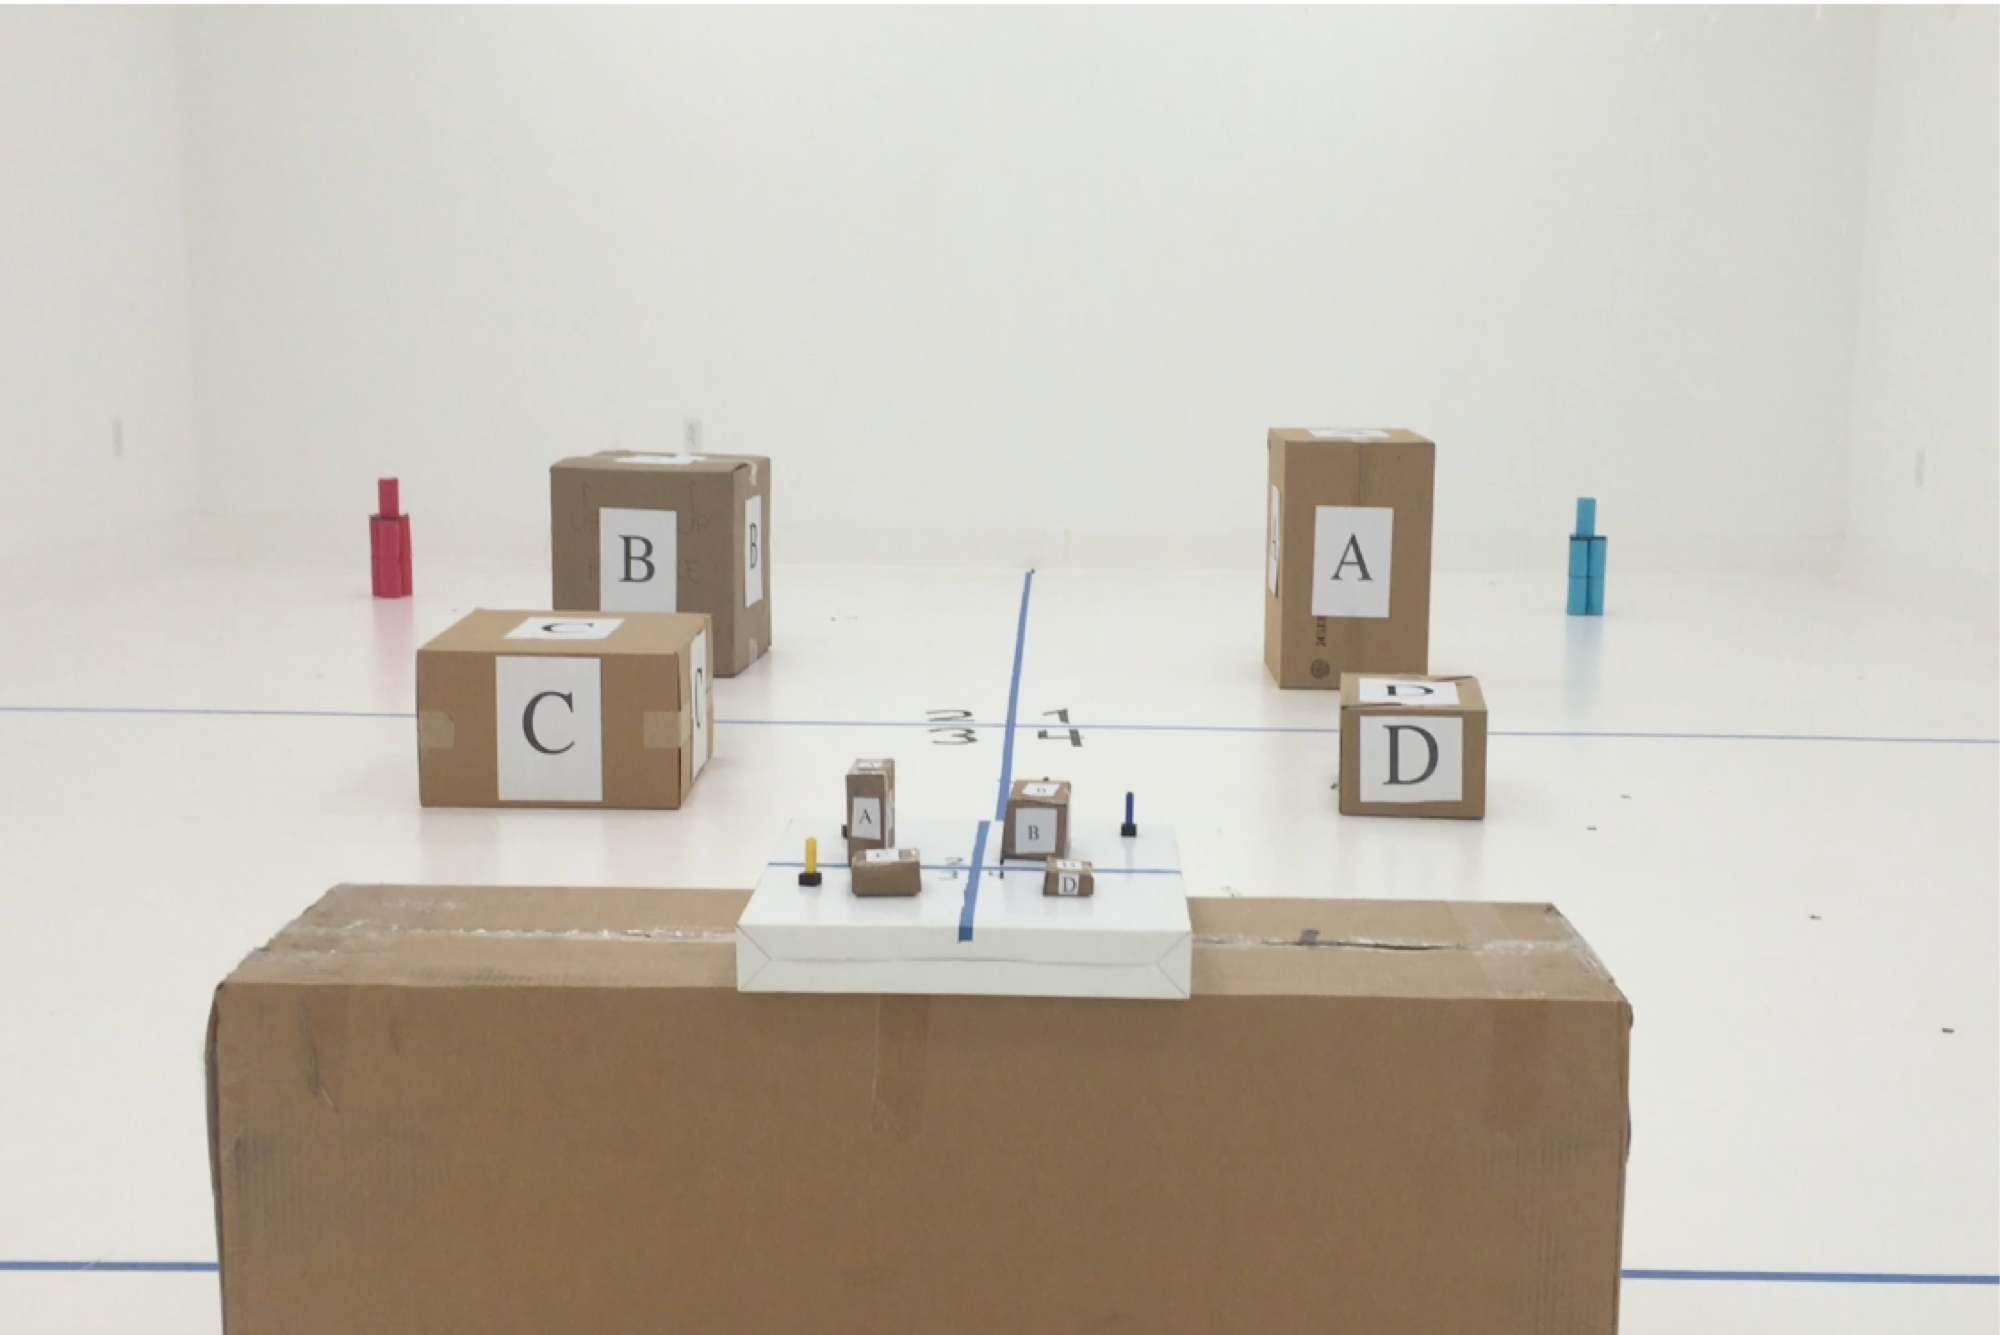
\includegraphics[width=.4\textwidth]{roomsetup}
\caption{Experiment room, including diorama. % and  most full-sized
                                % objects.
}\label{fig:roomsetup}
\end{figure}
%% \begin{figure}
%% \centering
%% 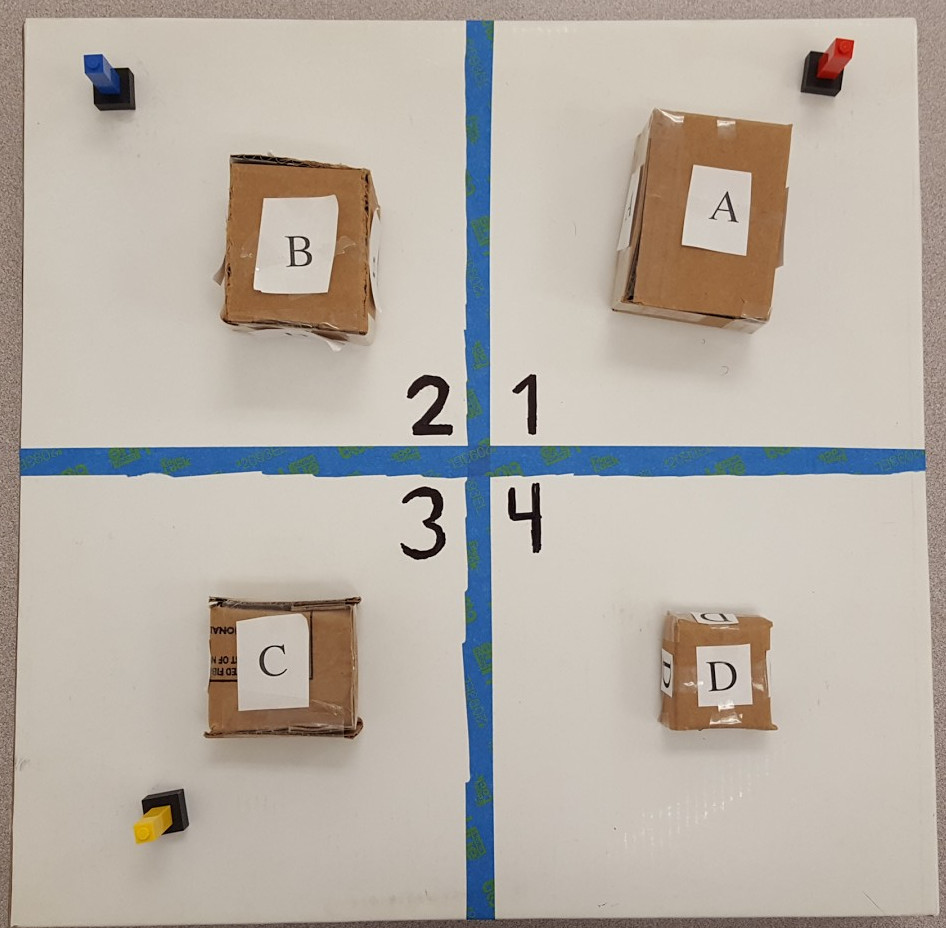
\includegraphics[height=0.45\linewidth]{Diorama1.jpg}
%% 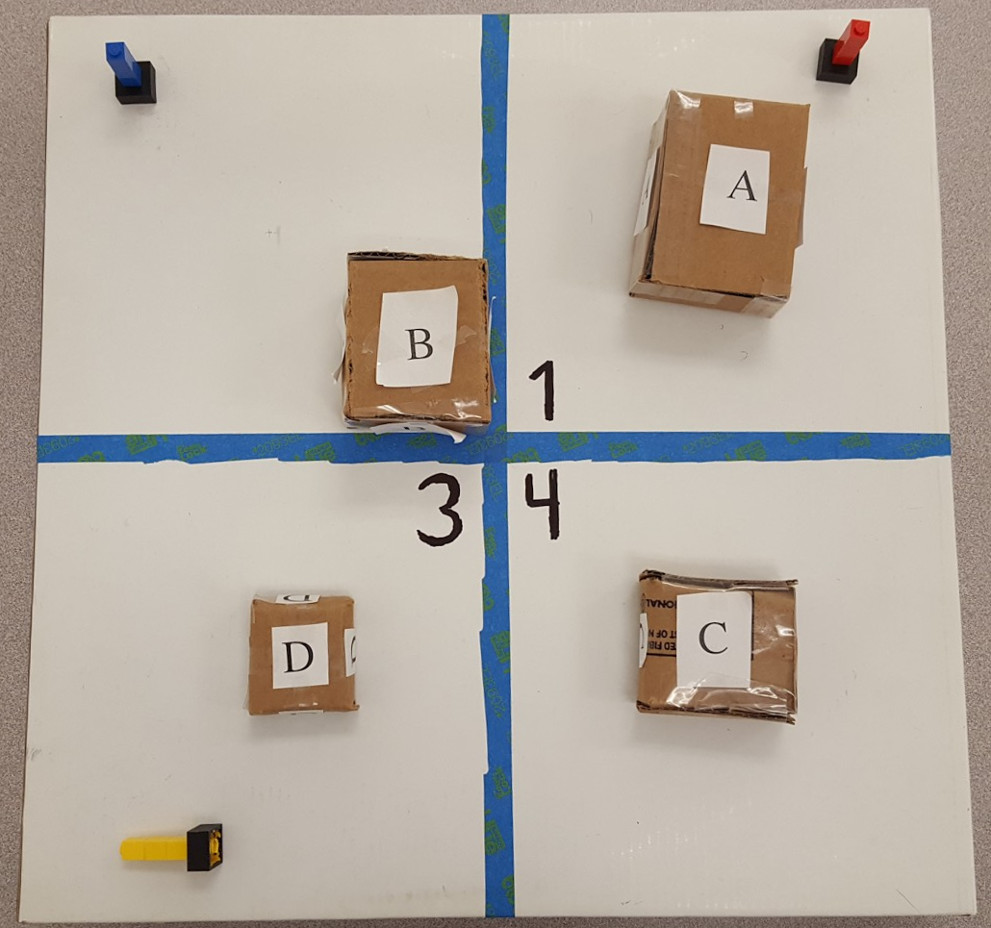
\includegraphics[height=0.45\linewidth]{Diorama2.jpg}
%% \caption{Starting diorama and example arrangement.}\label{fig:diorama}
%% \end{figure}
After participants finished arranging their diorama however they
wished, the researcher retrieved the first agent.
%% one of the agents (either 
%% robot or human, depending on agent order)
%% As the agent entered the
%% room, the researcher closed the door behind, and
The agent moved in
front of the participant, %% . The agent began the interaction by
introduced themselves, and stated ``Today I will be listening to
your instructions to arrange this room in the manner you have done
here,'' gesturing towards the participant's diorama. Participants then gave
instructions to the agent to arrange the full-size objects to
replicate their diorama arrangement, and the learner complied to the
best of their ability. Both human and 
robot learners restricted their utterances to ``Okay'', ``Yes'', and
``No'' whenever possible. The robot's utterances were selected by a human confederate,
and synthesized using a text-to-speech interface.  
Once the interaction was over, the agent said ``Goodbye'' and exited.  

\subsection{Teleoperation Interfaces}
%Let us now highlight
%%% Before we discuss the hypotheses this experiment was designed to test,
%%% we would like to highlight
%several decisions made as part of this
%experimental design.
There were several key decisions made as part of this work's experimental
design in order to facilitate ease of interaction, and minimize 
variability between participants. 
First, in order to ensure participant engagement,
naturalness of interaction, and prevent bias of the experimenter on
participants' utterances, 
participants in this experiment had
\emph{free control} over their arrangements and how those arrangements were
described (c.f.~\cite{schreitter2014exploring,SCHREITTER16.343}).
\begin{figure}
\centering
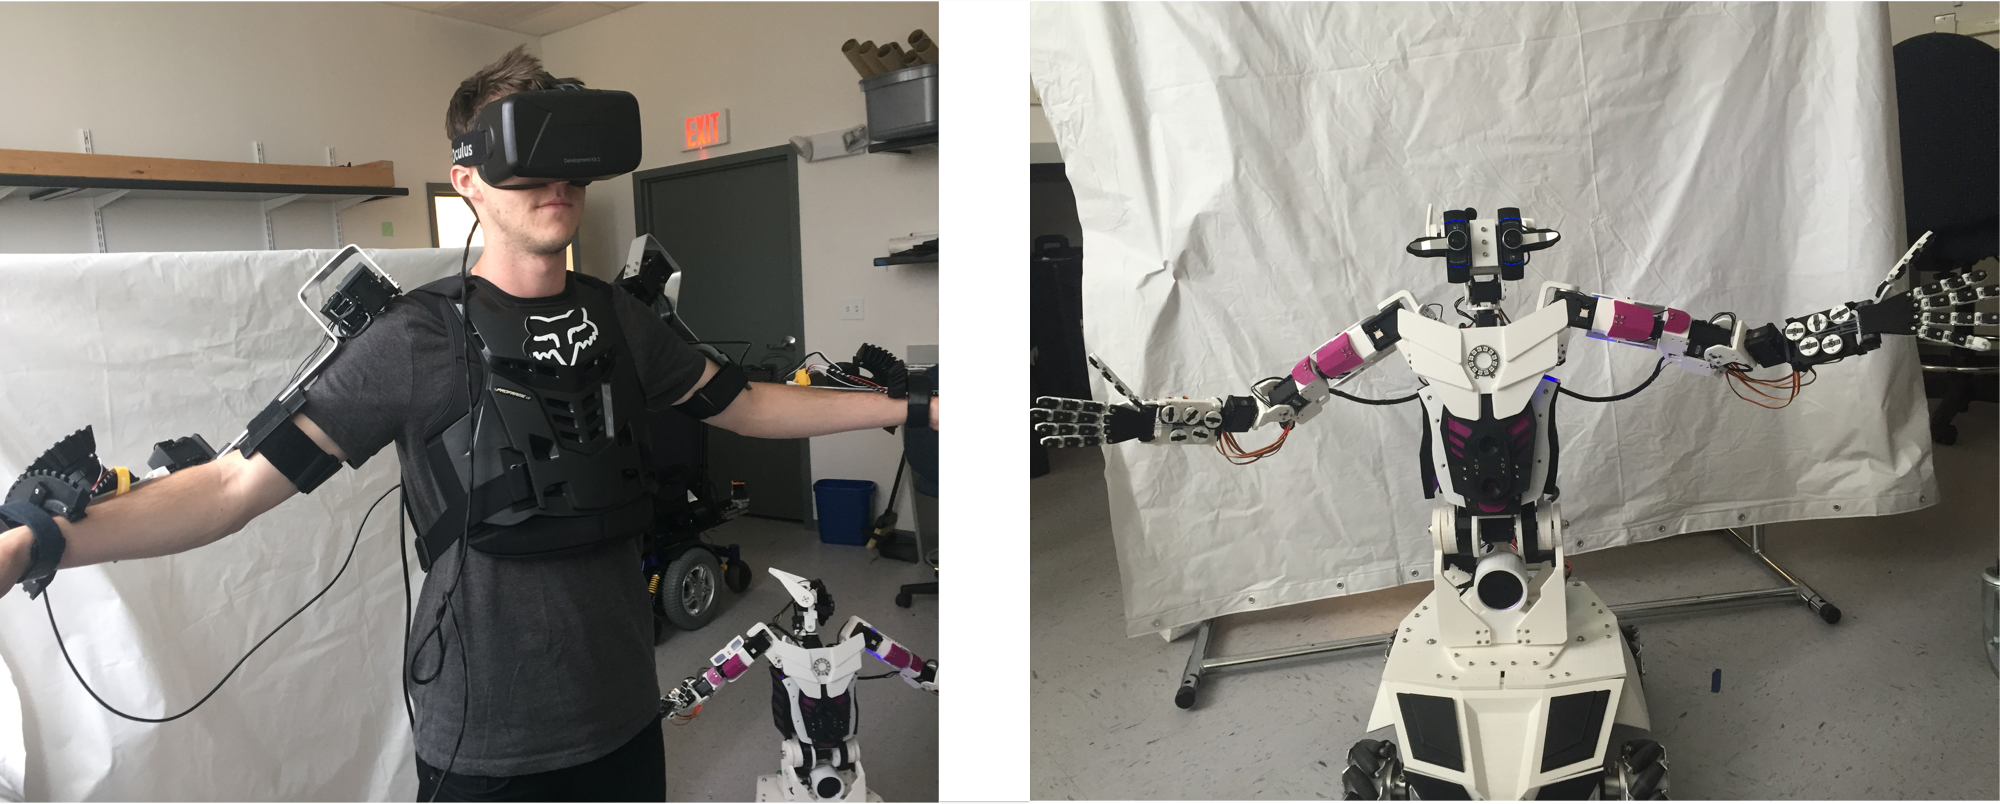
\includegraphics[width=.5\textwidth]{suitandpris}
\caption{Teleoperation exo-suit and humanoid robot. %used in the
                                %experiment.
}\label{fig:suitandpris}
\end{figure}
%
Second, a major key to this experiment was the specific robot and the 
control interface used: %% In this experiment, we used
a humanoid robot and a one-to-one exo-suit developed by
Kindred, as seen in Fig.~\ref{fig:suitandpris}. 
%% Both robot and exo-suit 
%% were made with a combination of 3-D printed materials, hobby
%% electronics, and off the shelf components.

This robot, 
%colloquially referred to as a QT (a reference to the science fiction
%writer Issac Asimov's short story, "Reason"), 
 made with a combination of 3D printed joints and limbs connected
by hobbyist servos, has 5 degree-of-freedom (DoF) arms, 10
under-actuated fingers (a plastic prosthetic hand model), and a 
2 DoF head. The robot's torso contains a small
computer and WiFi 
adapter for wireless communication, and its' base contains a battery to power the robot for several hours untethered.

Importantly, the robot and exo-suit 
were coupled with an Oculus Rift virtual reality headset so that a
human operator could be visually immersed 
in the robot's environment, using the stereoscopic cameras on the
robot as the video feed for the human operator. Additionally, two
microphones on the robot's head delivered stereophonic auditory 
data
so that language and sounds could be spatially localized even if the
audio source was not in the robot's line of sight. A set of 3 pedals
were used to move the 4-wheeled base of the robot.

Lastly, to standardize language and voice used throughout
the study, the robot's voice output was controlled by a second 
operator using a 
limited text-to-speech interface which allowed the robot to utter 
the
same introductory phrases and limited responses used by the 
human confederate.

%% . This interfaces allowed the robot to
%% utter, in addition to a few introductory phrases, a small set of
%% command responses such as ``Yes', ``No'', ``Okay'', and ``Sorry, I
%% didn't understand that.''





%% %%%%%%%%%%%%%%%%%%%%%%%%%%%%%%%%%%%%%%%%%%%5


%% We made use of a novel one-to-one immersive telepresence system
%% designed by \textit{ANONYMIZED} in order to maximize the overlap
%% between tasks that could be achieved by the human and the robot, and
%% in order to maximize the similarity between how the human and the
%% robot achieved those tasks. A Wizard-of-Oz interface was used solely
%% for controlling the speech output of the robots in both experimental
%% conditions in order to control the naturalness of the language used by
%% the robots across experimental conditions. 



%% %%%%%%%%%%%%%%%%%%%%%%%%%%%%%%%%%%%%%%%%%%%5

%% We gave each participant agency over the specific
%% tasks and instructions necessary to communicate in each
%% interaction, and by using the third-party's novel, one-to-one,
%% immersive telepresence system, we knew that any allowable action or
%% task could be completed by the humanoid robot and by the human. By
%% using a text-to speech interface for both the perceived autonomous and
%% perceived teleoperated interactions, we dissociated human-sounding
%% language from the teleoperated system and therefore produced a robot
%% that is as believeably autonomous as it is 
%% teleoperated.


%% TW: I don't understand the relation between interpretation of
%% robot and human errors, and the effect on blame -- furthermore, is
%% that something we investigated at all? *why* people believe errors
%% are committed?
%%------------------------------------------------------------------
%%  In the case of the present
%% research, we were aware that while the tasks of the study could be
%% fully completed by the robot and the human, the robot would not be
%% able to complete the tasks as efficiently and precisely as the human,
%% and thus, the mistakes and imprecision of the robot's task completion
%% would be attributed as either: a small human error in the teleoperated
%% condition, or as a major flaw of the system in the autonomous
%% condition. We thus hypothesized \textbf{(H3)} that the teleoperated
%% robot would be perceived as more successful at completing the task
%% than the autonomous robot.  

%% TW: How does this relate to the measures we collected?
%%-------------------------------------------------------
%% \textbf{(MB note to self: this relates to the idea that robots are able to do a few things repeatedly very well, so if it fails on one of these tasks it's indicative that the whole task is not possible for the robot, not just a singular, anomalous mistake).}

%% Humans talk in high-level language all the time, and previous research
%% in this area shows a high usage of Indirect Speech Acts
%% (ISAs)\cite{wilske2006service}. Because of the
%% frequent use of indirect language in human to human conversation, we
%% hypothesized \textbf{(H1)} that participants would talk in more
%% high-level language and use less low-level, direct, commands to the
%% teleoperated robot and the human than they would to the autonomous
%% robot. 


%Previous research has shown that humans more often utilize low-level, direct commands when speaking to autonomous agents than they do with humans .\footnote{related work: Study with specific, direct commands necessary for teaching robot playing soccer:\url{ftp://ftp.itam.mx/pub/alfredo/PAPERS/WRDRoboCupSymp2008.pdf}; \url{http://www.sciencedirect.com/science/article/pii/S0921889014002164}; \url{https://hrilab.tufts.edu/publications/briggsscheutz15aaaifs.pdf}}
%
%
\subsection{Experimental Procedure and Participation}
%% \begin{figure}[ht]
%% 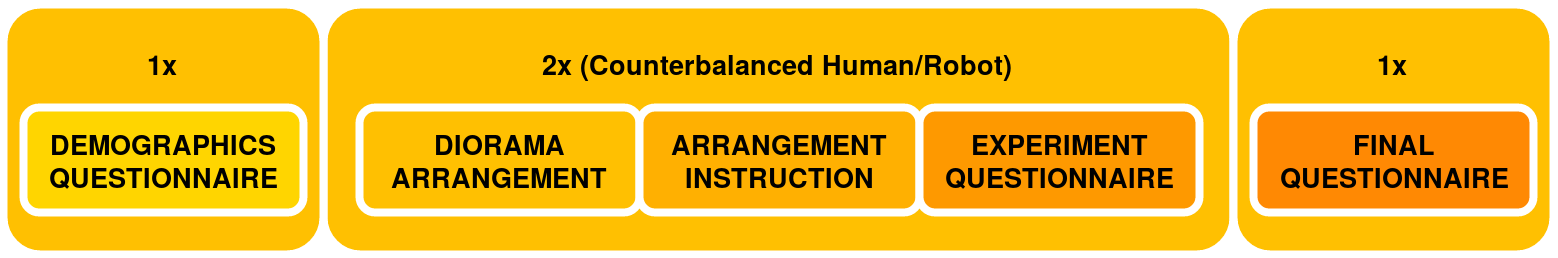
\includegraphics[width=0.5\textwidth]{IROS_PROCEDURE-1.png}
%% \caption{Experimental Procedure}\label{fig:procedure}
%% \end{figure}
%
%We will now discuss our experimental procedure. (Fig.~\ref{fig:procedure}).
Participants first completed a questionnaire 
gathering information on participants' demographics and  
previous 
experience with robots. All questionnaires were carried out in a
separate survey room. 
Participants then moved to the experiment room and conducted the main task. 
Next, 
participants 
completed a questionnaire
assessing their perceptions of the agent and the success of the task.
After completing this questionnaire, participants 
were told they would perform the
same task with ``another agent'' and that they were again free to
arrange their diorama however they wished. % (with the same few restrictions). 
Participants were not 
told what type of learner they would interact with next, but in all
cases the type of learner varied to counter the first interaction; if
a robot learner was used in the first experiment, a human learner was
used in the second, and vice versa. Upon finishing the second
interaction, participants answered the experiment questionnaire again,
as well as additional questions comparing the two tasks and agents.


Thirty-three students and university employees were recruited through fliers and
university class forums. Participants (21 Female, 12 Male) ranged in
age from  18 to 25 (M=20.85, SD=1.37). All participants were % and were 
%% Participants were 
given \$10 as compensation for their time. % for their time.
% (approximately 30-45 minutes). 


\subsection{Measurement}
In addition to the demographic survey, as previously described,
questionnaires were used to
assess participants' perceptions of their human and
robot teammates. 
Participants' perceptions varied along a variety of dimensions,
including cooperativity, capability, annoyingness, creepiness, and
responsiveness
%% belief \textit{before} meeting the learner that the learner would be capable of replicating the
%% participant's block arrangement (1=``strongly disagree'' to
%% 7=``strongly agree''), attentiveness, gaze-following,
%% tendency-to-ignore, understanding, belief \textit{after} meeting
%% the learner that the learner would be capable of replicating the
%% participant's block arrangement (1=``no'' to 7=``yes''), arrangement
%% complexity (1=``simple'' to 7=``very complex''), ease of interaction
%% (1=``easy'' to 7=``hard''), level of comprehension (1=``low'' to 7=``high''), and
%% successfulness (1=``completely unsuccessful'' to 7=``very successful'').
%% Finally, participants were asked to imagine if, in an alternate interaction with the robot, they believed that the robot would have been capable of
%% understanding three commands within that new task.

%% Finally, participants were asked to imagine that the four boxes had
%% been blocks of different colors, and asked them whether they believed
%% the learner would have understood a variety of commands:
%% ``Did you think the learner would have understood you if you told them
%% to `move the red block to the right of the blue block'?," ``Do you
%% think the learner would have understood you if you pointed at part of
%% your arrangement and told the learner to `arrange the blocks like
%% this'?," and ``Do you believe the learner would have understood you if
%% you had said `do the same thing but with the green block'?" 

In addition to these subjective, self-reported measurements, we also
collected several objective behavioral measures. For each participant, video
recording was used to assess the number of words used by participants,
%percentage of directives in which participants grouped multiple
%instructions into a single directive, 
and the percentage of
utterances used by 
participants that were ISAs, as well as the
complexity of participants' arrangements, as described in our previous
work~\cite{bennett2017differences}.
%% , as assessed by the
%% metric discussed below. Arrangement complexity
%% was calculated to use as a covariate in our analyses, as we are
%% interested in the indirectness of participants' utterances and the number
%% of words required to accomplish the given tasks
%% \emph{regardless of task complexity}. For example, using an
%% external complexity estimate as a covariate will allow us to control
%% for the fact that more complex tasks 
%% likely require more words to complete. 

%% Arrangement complexity was calculated as
%% $(b_0+b_1+b_2+b_3)+(t_0+t_1+t_2)+s$, where each box
%% $B_i$ contributed $b_i$ points if moved (equal to the number of
%% centimeters moved within the diorama), each tower $T_i$ contributed
%% $t_i$ points if knocked down (equal to one-half its distance from the
%% center of the diorama), and a ``systematicity bonus'' $s$ was added
%% equal to the smallest number of groups $c_0,...c_n$ that
%% could be formed by grouping the boxes by symmetry of
%% motion\footnote{For example, all four boxes moving one quadrant
%% counter-clockwise yields one group; two boxes rotating counter-clockwise and
%% the others not moving yields two groups; two boxes rotating counter-clockwise, one box
%% not moving, and one box moving to the far right of its
%% quadrant yields three groups; one box
%% rotating counter-clockwise, one box not moving,
%% one box moving to the far right of its quadrant, and one box moving to
%% the center corner of its quadrant yields four
%% groups. }, as depicted in Fig.~\ref{fig:dioramac}.
%Note that this is only intended as a means to
%estimate complexity within this experiment, and is not intended for
%use beyond this experiment.


%% Arrangement complexity was calculated
%% as follows: each cardboard box contributed $b$ points towards the
%% complexity score, where $b$ was the number of centimeters the box
%% moved from its starting position to its ending position in the
%% diorama; each tower of cans knocked over contributed $t$ points
%% towards the complexity score, where $t$ was one-half the distance in
%% centimeters from the center of the room to the position of the can in
%% the diorama; finally, a ``systematicity bonus'' $c$ was added to each
%% score, where $c$ was the smallest number of groups that could be
%% formed by grouping the motion of the cardboard boxes by symmetry of
%% motion. 
%
%% \begin{figure}
%% \centering
%% 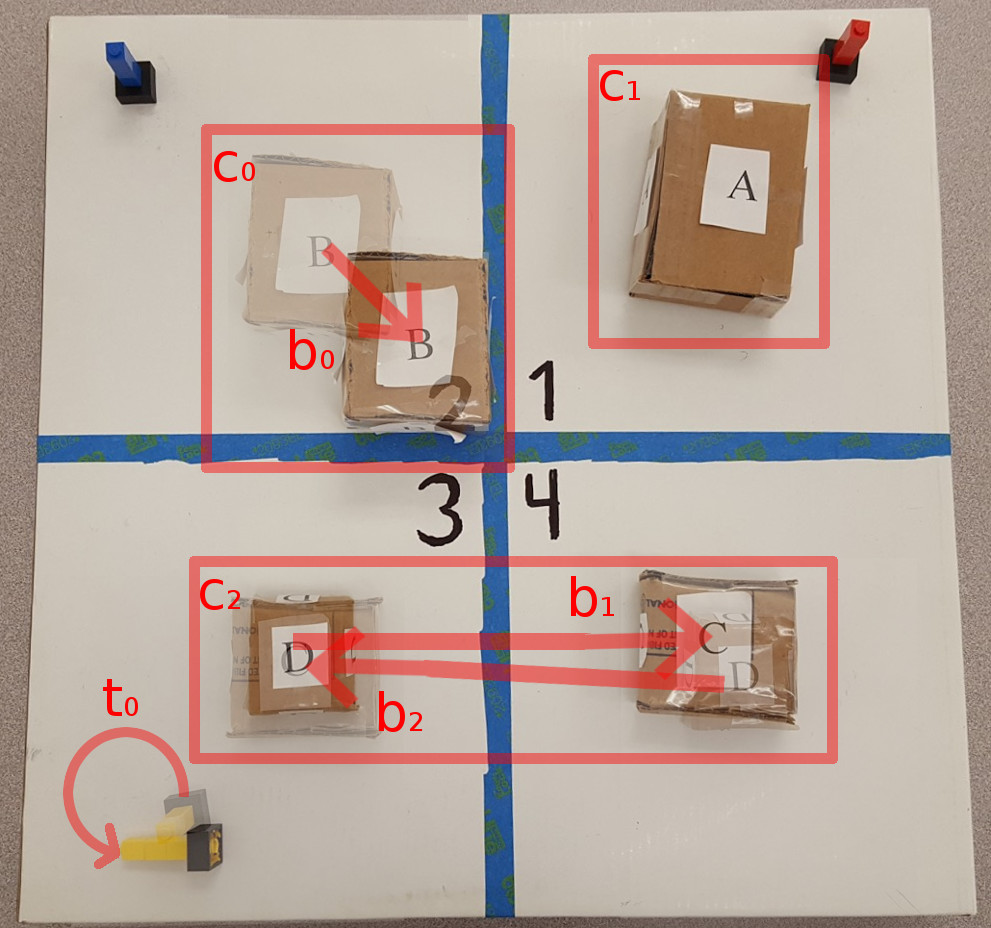
\includegraphics[width=0.28\textwidth]{DioramaC.jpg}
%% \caption{Sample complexity diagram for Fig.~\ref{fig:diorama}
%%   arrangements.
%%   %shown
%%   %in . %% Here, each box contributed an
%%   %% amount equivalent to the length of complexity would be
%%   %% calculated as $b_0+b_1+b_2+t_0+c_0+c_1+c_2$, where $b_i$ is the
%%   %% length of the shown arrow, in centimeters, $t_0$ is one-half the
%%   %% distance from the yellow tower to the center of the diorama, in
%%   %% centimeters, and $c_i$=1.
%% }\label{fig:dioramac}
%% \end{figure}
%
\section{Results}
\label{sec:results}
In this section we provide a brief summary of our experimental
results. We refer the interested reader to our full results described
in our previous work~\cite{bennett2017differences}. 

%% \subsection{Objective Measures}

%Analysis of our collected data showed that in \textbf{AC}, 70.59\% of participants
%used at least one ISA when directing another human but only 29.41\% of
%participants used one when directing a robot, while in \textbf{TC}, 50.0\% of participants used at least one ISA when speaking with another human, but 56.25\% of participants used
%at least one when speaking to the teleoperated robot.

Participants used significantly more words to describe the task in the
\textbf{TC} (M=204.88, SD=181.60) than in \textbf{AC} (M=72.82, SD=42.83), F(1,29)=8.05, p=.008. An ANCOVA using task complexity as a covariate 
attenuated this effect, F(1,29)=4.43, p=.02. 
%
%% \begin{figure}
%% \centering
%% 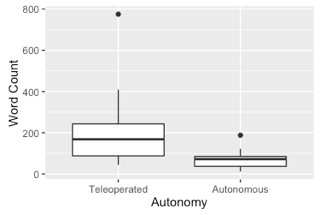
\includegraphics[width=0.7\linewidth]{Boxplots/WordCount.png}
%% \caption{Effect of autonomy on participant verbosity}\label{fig:wca}
%% \end{figure}
%
Additionally, %% a significant difference was found with respect to the
%% number of words used by humans to describe the task to all learners:
%The results suggest that 
participants used more words to describe the
task (to either learner) in \textbf{TC}
(M=153.28, SD=103.40) than
in \textbf{AC}(M=80.09, SD=40.02), F(1,29)=6.91, p=.014,
an effect attenuated in a subsequent ANCOVA,
F(2,62)=4.72, p=.012. An interaction between
condition and learner was also found: far more words were used with
robots in \textbf{TC}
(M=204.88, SD=181.60) than with \textit{humans} in \textbf{TC}
(M=101.69, SD=44.79), robots in \textbf{AC} (M=72.82,
SD=42.83) or humans (M=87.35, SD=46.27) in
\textbf{AC}, F(1,29)=7.79, p=.009, an effect that was
strengthened in a subsequent ANCOVA, F(6,58)=3.25, p=.008.

%% No significant difference was found in the proportion of user-directed
%% utterances that used metric-level commands
%% (e.g., moving a certain direction for a certain amount of time)
%% vs. higher-level commands.

%% \subsection{Subjective Measures}
%% \subsubsection*{Differences by Purported Autonomy}
%% In this section, we will describe differences we found between
%% \textbf{AC} and \textbf{TC}. %% when
%% %% participants were told that robot learners would be AUTONOMOUS vs. TELEOPERATED.
%
%% Participants in \textbf{AC}
%% judged their arrangements to be less complex in 
%% retrospect (M=2.53 SD=1.28) after interacting with robot learners
%% than did participants in \textbf{TC}
%% (M=4.00, SD=1.37), F(1,29)=9.92, p=.004. When arrangement complexity
%% was treated as a covariate in a subsequent analysis of covariance,
%% this effect was attenuated, F(2,29)=5.92, p=.007.
%
%% Participants in \textbf{AC} less
%% strongly agreed that robots could be conscious (M=3.06, SD=1.78) than
%% those in \textbf{TC} (M=4.38, SD=1.59),
%% F(1,29)=5.60, p=0.025, 
%% %
%% and less strongly believed that the robot learner had been following their
%% gaze (M=4.06, SD=1.49) than did participants in \textbf{TC} (M=5.09, SD=1.19), F(1,29)=5.43, p=.027.

%% \subsubsection*{Differences by Agent}
Furthermore, a number of significant differences were found
between perceptions of the human learners and the robot
learners:%, as seen in Tab.~\ref{tab:diffAgent}:
%
%%  Participants rated human learners to be slightly more
%% capable (M=6.88, SD=0.33) than robot learners
%% (M=5.97, SD=1.04), F(1,29)=28.07, p$<$.001 (as seen in Fig.~\ref{fig:capa}), 
%% %
%% \begin{figure}
%% \centering
%% 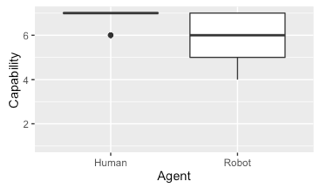
\includegraphics[width=0.7\linewidth]{Boxplots/Capable(Agent).png}
%% \caption{Effect of agent on perceived capability}\label{fig:capa}
%% \end{figure}
%
%% rated human learners as slightly
%% less annoying (M=1.36, SD=0.93) than they did robot learners (M=2.00, SD=1.17),
%% F(1,29)=7.02, p=.013, 
%% %
%% less creepy
%% (M=1.67, SD=1.08) than they did robot learners (M=2.73, SD=1.72), 
%% F(1,29)=11.16, p=.002, 
%% %
%% more conscious
%% (M=6.97, SD=0.17) than they did robot learners (M=3.97, SD=1.78), 
%% F(1,29)=91.63, p$<$.001, 
%
%% and easier to interact with (M=2.06, SD=1.84) than
%% they did robot learners (M=3.15, SD-1.73), F(1,29)=6.67, p=0.015.
%
%
%
%% \begin{figure}
%% \centering
%% 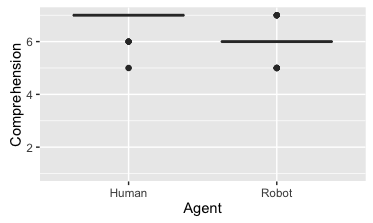
\includegraphics[width=0.7\linewidth]{Boxplots/Comprehension(Agent).png}
%% \caption{Effect of agent on perceived comprehension}\label{fig:compa}
%% \end{figure}
%% %
%% \begin{figure}
%% \centering
%% 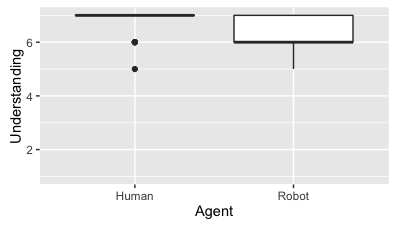
\includegraphics[width=0.7\linewidth]{Boxplots/Understanding(Agent).png}
%% \caption{Effect of agent on perceived understanding}\label{fig:unda}
%% \end{figure}
%
\begin{table}[ht]
\begin{small}
%\caption{Perceptions of Agents}\label{tab:diffAgent}
\begin{tabular}{l|llrr}
 & H(M, SD) & R(M, SD) & F(1,29)& p\\
\hline
Capable & 6.88, 0.33 & 5.97, 1.04 & 28.07,  & $<$.001\\
Annoying & 1.36, 0.93 & 2.00, 1.17 & 7.02 & .013 \\
Creepy & 1.67, 1.08 & 2.73, 1.72 & 11.16 & .002\\
Conscious & 6.97, 0.17&3.97, 1.78&91.63&$<$.001\\
Easy Interaction & 2.06, 1.84&3.15, 1.73&6.67&.015\\
Comprehension&6.76, 0.56&5.94, 0.66&29.45&.007\\
Understanding&6.79, 0.48&6.27, 0.76&12.96&.001\\
Gaze Following&5.42, 1.85&3.70, 1.84&17.07&$<$.001\\
Perceived Success& 6.78, 0.48 & 6.12, 0.93 & 12.99 & .001\\
\end{tabular}
\end{small}
\end{table}

%% Participants also more strongly agreed that human learners
%% comprehended them (M=6.76, SD=0.56) 
%% than did robots (M=5.94, SD=0.66), F(1,29) = 29.45, p$<$.007 (as
%% seen in Fig.~\ref{fig:compa}), 
%% %
%% more strongly agreed that human learners understood what they were
%% saying (M=6.79, SD= 0.48) than did 
%% robots (M=6.27, SD=0.76), F(1,29)=12.96, p=0.001 (as
%% seen in Fig.~\ref{fig:unda}),
%% %
%% and more strongly agreed that human learners had followed their gaze
%% (M=5.42, SD=1.84) than they believed that robots had (M=3.70, SD=1.84),
%% F(1,29)=17.07, p$<$.001.

%% Participants retrospectively reported more strongly predicting task success for human
%% learners both after meeting those learners (M=7.00 (SD=0) vs. M=5.27
%% (SD=1.48), F(1,29)=43.67, p$<$.001)
%
%% \textit{and before} meeting those learners (M=6.24 (SD=1.19)
%% vs. M=5.64 (SD=1.22), F(1,29)=8.16, p=.008). Participants accordingly
%% adjudicated higher task success when interacting with a human learner (M=6.78,
%% SD=0.48) than they did when interacting with a robot learner
%% (M=6.12, SD=0.93), F(1,29)=12.99, p=.001 (as
%% seen in Fig.~\ref{fig:succa}).
%
%% Participants were also less likely to believe that a
%% robot would understand each of the three alternate-scenario commands
%% than %% they were
%% that a human would, as seen in Tab.~\ref{tab:asc}:\\%, as seen in Tab.~\ref{tab:as} %% (M=5.15,SD=2.08 vs. 6.48
%% %\begin{table}
%% %\caption{Alternate scenario command understandability}\label{tab:as}
%% %
%% \begin{table}[ht]
%% \begin{small}
%% \caption{Alternate-Scenario Commands}\label{tab:asc}
%% \begin{tabular}{l|llll}
%%  & Human(M,SD) & Robot (M,SD) & F(1,29)& p\\
%% \hline
%% C1 & 4.67,1.99 & 5.76,1.79 & 9.16, & .005\\
%% C2 & 5.15,2.08 & 6.48,1.12 & 15.15 & $<$.001 \\
%% C3 & 2.85,1.84 & 6.70,0.92 & 105.27 & $<$.001\\
%% \end{tabular}
%% \end{small}
%% \end{table}
%% %
%% %% \begin{figure}
%% %% \centering
%% %% 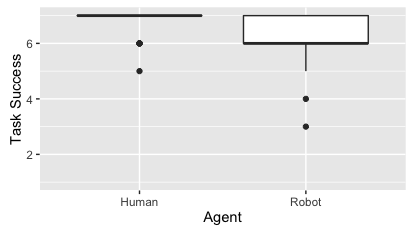
\includegraphics[width=0.7\linewidth]{Boxplots/Success(Agent).png}
%% %% \caption{Effect of agent on participant success}\label{fig:succa}
%% %% \end{figure}







%% %% ``Move the red block to the right of the blue
%% %% block'' (M=5.15, SD=2.08) than they were that a human would
%% %% (M=6.48, SD=1.12), F(1,29)=15.15, p<.001, slightly less likely to
%% %% believe that a robot would understand ``Do the same thing with the
%% %% green block'' (M=4.67, SD=1.99) than they were that a human would
%% %% (M=5.76, SD=1.79), F(1,29)=9.16, p=.005, and far less likely to believe that a robot
%% %% would understand ``Arrange the blocks like this'' (M=2.85, SD=1.84) than
%% %% they were that a human would (M=6.70, SD=0.92), F(1,29)=105.27, p<.001.

%% \subsubsection*{Interaction Effects}
%% A significant interaction between condition and learner was found on
%% adjudication of task complexity: Participants in \textbf{TC} %% the TELEOPERATED
%% %% condition
%% ranked the arrangements they gave to robots significantly
%% more complex (M=4.00, SD=1.37) than they did the arrangements they gave
%% to humans (M=2.93, SD=1.34) or the arrangements that participants in
%% \textbf{AC} gave to either robots (M=2.53, SD=1.28) or
%% humans (M=2.76, SD=1.09), F(1,29)=7.10, p=.012. This effect was
%% attenuated by a subsequent analysis of covariance, 
%% F(6,58)=2.62, p=.026.

\section{Discussion}
\label{sec:disc}

Throughout conducting this experiment and by way of using the exo-suit teleoperation interface for numerous hours, a number of challenges and learnings were made. Firstly, given that our experiment required real time remote communication via motor control, vision, and hearing, we found any spikes in latency to be extremely detrimental to the running of the experiment. A spike in latency might lead to: a participant's instruction not being heard, inaccurately executing a movement, or having to operate blindly (depending on the modality affected). With the technology used in this study, latency was not generally an issue unless there was high bandwidth usage or congestion on  back-end server calls. Future work might mitigate this issue by ensuring that high quality WiFi adapters are used, and that high bandwidth internet proliferates the experiment area.

Secondly, the size of the items we chose to move around the room were slightly too large in proportion to the size of the robot, which can be gleaned from Fig.~\ref{fig:suitandpris}. Although this choice was deliberate (wanting to maximize the size of items used by the robot so they wouldn't be trivial for the human to also use), it occasionally resulted in the teleoperater being unable to view the surroundings while controlling the robot, as the robot's peripheral
vision might have been obscured by the item.

Finally, there were a number of lessons learned about how this teleoperation mechanism affected our experiment design. Because we were using the same teleoperator, exo-suit, and robot for all of our trials, and because we had the capability of seeming exceptionally human-like (with fluid, complex movements, or advanced language), we had to ensure that in any and all trials the robot did not seem too human-like to be obviously perceived as teleoperated, nor too robotic to be obviously perceived as autonomous. Thus, the teleoperator used standardizing strategies such as keeping their arms on arm rests whenever possible, so that complex forearm movement did not expose the level of autonomy. Additionally, the text-to-speech interface and set of commands was used to mitigate any variability in language across participants, but this prescribed language did seem to force the human-human interactions to be more awkward than they would have been with more fluid language.


%% Our results suggest that participants perceived the robot as less capable and intelligent than the human, and spoke in more directive commands, which is in line with previous research and our hypotheses. Additionally, participants treated the teleoperated robot with more human-like capacities, such as attributing consciousness to the robot, and talking to the robot more. This evidence suggests that people conducting future robot design and HRI studies ought to heavily consider the ways in which they present the autonomy levels of robots as they strongly influence perceptions of robots and the interactions humans have with robots.


%% \textbf{(H2)} was confirmed as participants perceived the robot, teleoperated \textit{and} autonomous, to be less capable, to not have understood their instructions as well, and upon first seeing the robot, thought it would not be successful at completing the task. Additionally, participants thought humans were dramatically more likely to understand phrases with indirect language, such as ``arrange the blocks like this." 

%% Furthermore, some interesting data was gathered around single command usage in our behavioral analysis of participants' interactions. Participants used 10\% more single commands directed towards the robots, autonomous and teleoperated, than they did to the humans; perhaps more interestingly, though, was the discovery that for the participants who first interacted with a human, when interacting with the robot after they used 20\% more single commands. While this may in part be due to participants understanding the goals of the task after completing their first interaction and thus trying to expedite the study's completion by quickly commanding the robot, participants who interacted with a robot first do not exhibit the same increase in single-command usage. Thus, it seems that the robotic agent in particular lead to an increased use of single, directive, commands, likely due to the perception of decreased capacity for understanding complex language.

%\begin{enumerate}
%\setcounter{enumi}{2}
%\item On perceived understanding, a significant effect of Agent. Means: Human (6.79), Robot (6.27) (p$\approx$0.0012)
%\item On perceived capability, a significant effect of Agent. Means: Human (6.88), Robot (5.97) (p$\approx$0.000011)
%\item On retrospective reports of whether participants thought the agent would be successful after meeting them, a significant effect of Agent  (p$\approx$0.0000003). Means: Human (7.00), Robot (5.27). 
%\item a significant effect of Agent on decision of whether the learner would have understood ``arrange the blocks like this" (p$\approx$0.00000000003). Means: Human (6.70), Robot (2.85).
%\item a significant effect of Agent on decision of whether the learner would have understood ``do the same thing with the green block" (p$\approx$0.005). Means: Human (5.76), Robot (4.67) 

%We hypothesized \textbf{(H1)} that participants would use
%more indirect language when communicating with robots in \textbf{TC}
%than they would in \textbf{AC}, but less than 
%when communicating with other humans. We did not find any evidence
%suggesting that participants used a higher \textit{proportion} of
%ISAs when speaking with humans, but found that
%the use of a purportedly autonomous robot (whose use reinforced the
%difference in human-likeness between human-and-robot) may have caused
%participants to be more likely to use indirect language \textit{at
%  all} when directing their human teammate, and less likely when
%directing the robot. Overall, however, the lack of a significant
%difference in overall ISA use between humans and
%robots reinforces the importance of enabling robots to understand
%these types of utterances. In fact, some participants
%\textit{exclusively} used ISAs, even when directing a
%purportedly autonomous robot.

%% (Fig.~\ref{fig:trans1}):
%% \begin{figure}[ht]
%% \begin{center}
%% \fbox{\parbox{0.95\linewidth}{
%% \begin{description}[noitemsep,topsep=0pt]
%% \small
%% %\itemsep0em 
%% \item[H:]Alright Alex, can you take the box B... D over there in quadrant 4 and move it to quadrant 3?
%% \item[R:]OK.
%% \item[H:]Can you move the box D to your right of box C?
%% \item[R:]OK.
%% \item[H:]Um... can you move it to the other side of box C?
%% \item[R:]OK.
%% \item[H:]Perfect.
%% \item[H:]Can you go to quadrant 2 and knock over the red tower?
%% \item[R:]OK.
%% \item[H:]Um can you go to quadrant 1 and knock over the blue tower?
%% \item[R:]OK.
%% \item[H:]It's all done.
%% \end{description}
%% }}
%% \end{center}
%% \caption{\small Transcript excerpt: human instructing ``autonomous'' robot}\label{fig:trans1}
%% \end{figure}
%% %


We hypothesized \textbf{(H1)} that not only would robots described to
participants as \textit{autonomous} be perceived as less
intelligent and capable than humans would be, but also that robots described
to participants as \textit{teleoperated} would be perceived with similarly diminished capabilities, even though
in reality all three learners had identical cognitive capabilities. In
fact, this is just what we observed. Our results showed that
participants rated both autonomous \emph{and teleoperated} robots as less understanding of their
instructions and less likely to understand high level commands.
% such as
%``Arrange the blocks \textit{like this}' (C3). 
This is striking, as such
ratings should depend only on the \emph{mental faculties} of the
learner, and yet, participants rated the human-teleoperated robot no
differently in this respect than they did in \textbf{AC}. Furthermore, both autonomous \textit{and teleoperated} robots 
were rated as more annoying, creepy, harder to interact with, and
overall less capable \textit{and conscious} than their human counterparts.

This suggests that regardless of whether or not a robot is
human- or AI-controlled, humans are likely to see the robot's form as  
hindering its controller's capabilities \textit{and intelligence}.
%%  a
%% finding with significant implications for robot designers. 
This is particularly significant for human-robot collaboration, as it
suggests that people may view not only a teleoperated robot, but also
\textit{its teleoperator}, as inferior to a present human counterpart, altering
both social dynamics and expectations of success.  
%
%% In our experiment, such effects can be observed in
%% exchanges such as that seen in Fig.~\ref{fig:trans2}:
%% %
%% \begin{figure}[ht]
%% \begin{center}
%% \fbox{\parbox{0.95\linewidth}{
%% \begin{description}[noitemsep,topsep=0pt]
%% \small
%% \item[H:] Turn right 90 degrees
%% \item[H:] Go forward point-two-five seconds
%% \item[H:] Turn right 90 degrees
%% \item[H:] Push box point-two seconds
%% %\item[H:] Straighten box 
%% \end{description}
%% }}
%% \end{center}
%% \caption{\small Transcript excerpt: human instructing teleoperator.}\label{fig:trans2}
%% \end{figure}
%
%Especially concerning to us was one subject whose use of direct
%commands when interacting with a robot teleoperator carried over into
%interactions with a co-present human teammate:

%% What is especially concerning here is not only that this
%% participant used direct, low-level language to command a (fellow
%% human) teleoperator, but also that
%% %the participant's use of this language then
%% these patterns
%% carried over into his second interaction, now with a
%% \textit{co-present human teammate}, as shown in Fig.~\ref{fig:trans3}:

% -- an observation we find particularly troubling. 
%\begin{figure}[ht]
%\begin{center}
%\fbox{\parbox{0.95\linewidth}{
%\begin{description}[noitemsep,topsep=0pt]
%\small
%\item[H:] Move box B towards the wall, uh, point-two seconds.
%\item[H:] Move box B away from the line half a second.
%\item[H:] Turn box B 45 degrees.
%\end{description}
%}}
%\end{center}
%\caption{\small Transcript excerpt: human instructing co-present
%  human.}\label{fig:trans3}
%\end{figure}
%% Future research in this area might focus on understanding what
%% aspects of the robot's appearance and behaviors influence this
%% belief, e.g. its size or its fluidity of movement, and how a
%% teleoperator's humanness could be best reinforced.
%% Additionally, future exploration might also investigate how augmenting a
%% teleoperated robot with some super-human capabilities or unique
%% knowledge (that the interacting human does not posses) might influence
%% perceptions of both robot and teleoperator.

Finally, because higher levels of autonomy have previously been correlated with
higher levels of blame and scrutiny, we hypothesized \textbf{(H2)}
that autonomous robots would receive less credit for successful
completion of the task than would teleoperated robots (i.e., that teleoperated
robots would be rated as more successful). While we did not find
evidence supporting this hypothesis, we did observe that participants
in \textbf{TC} 
retrospectively judged the arrangements provided to robot learners to
be more complex than did participants in \textbf{AC},
even when controlling for the actual complexity of their
arrangements. This suggests that participants may have attributed more
of the credit for task success to the \textit{learner} in \textbf{TC},
but to have retrospectively assumed \textit{simplicity
  of arrangement} in \textbf{AC}, which would indirectly
support H2.


%% was also found, though not as directly as with the evidence for
%% \textbf{(H2)}. Participants who interacted with the teleoperated robot
%% retrospectively judged their arrangements as more complex than people
%% in the autonomous condition did. One reason for this being the case
%% could be that participants in the teleoperated condition had
%% expectations that the human-controlled-robot should not have any
%% issues replicating the diorama, and thus when the robot's precision
%% was not exact and speed was slower than humans, these participants
%% rated their arrangement as more difficult. In the autonomous
%% condition, however, expectations or performance were less tied to any
%% pre-concieved notions, and thus these participants fell into the
%% perspective that: the arrangement was easy but the robot just couldn't
%% do it. Similarly, participants may have seen mistakes of the robot in
%% the autonomous condition as indications of bad control algorithms or
%% flaws in the overall system, whereas imprecision and mistakes in a
%% human-controlled, teleoperated robot are just human error and less
%% indicative of capability. 


%% TEW -> MB: How does this relate to H3?
%% -------------------------------------------------------------------
%% Additionally, participants in the autonomous condition believed less
%% strongly that ``robots can be conscious" after interacting with the
%% robot. One reason for this may again fall on differing pre-conceived
%% notions of the teleoperated robot vs. of the autonomous robot: in the
%% autonomous condition, participants are expecting lower performance,
%% and are quicker to see mistakes and imprecision as indicative of lower
%% capabilities and thus lower capacity to be conscious. 


%% The differing
%% perceptions we observed of autonomous and teleoperated robots performing the same
%% task reinforces the importance of ensuring that humans are 


%% humans of the autonomy level or control type of the robot, as they may
%% be more forgiving of robot mistakes if they know a human remotely
%% operating. Additionally, it may be important to strategically not
%% inform humans of a robot's level of autonomy if there is high
%% potential for mistakes and if a diminished perception of capability
%% could influence the interaction with that robot. 





%% We found no evidence to support
%% this hypothesis, which suggests that the extent to which humans will
%% use indirect language when communicating with robots may be higher
%% than previously thought. Previous evidence has suggested that humans
%% use indirect language more frequently in contexts with
%% conventionalized social norms. In this experiment, however,
%% participants used indirect language with robots just as frequently as
%% with humans. On the other hand, clear differences in communication
%% were observed in the experiment: participants were much
%% more verbose in the TELEPRESENCE condition when speaking with the
%% robot, 
%% % yet also more likely to provide all parts of their instructions
%% % in a single utterance rather than split into steps
%% suggesting that
%% interactions with teleoperated robots will indeed 
%% strongly differ from those humans have with other humans or with
%% robots they believe to be autonomous.


%% \textbf{not sure if this is more in support of H2 than H1, but is language related}
%% Additionally, some interesting data was gathered around single command usage. Participants used 10\% more single commands directed towards the robots, autonomous and teleoperated, than they did to the humans; perhaps more interestingly, though, was the discovery that for the participants who first interacted with a human, when interacting with the robot they used 20\% more single commands. While this may in part be due to participants understanding the goals of the task after completing their first interaction and thus trying to expedite the study's completion by quickly commanding the robot, participants who interacted with a robot first do not exhibit the same increase in single-command usage. Thus, it seems that the robotic agent in particular lead to an increased use of single, directive, commands.

%% These findings also have important implications for future human-robot interaction research and robot design. As previously mentioned with findings from H3, robot designers and researchers may want to selectively inform or hide information about the level of autonomy of a robot to control human perceptions of capability and intelligence. This same takeaway applies here to language as well; if humans need to speak in certain manners to robots so that an autonomous algorithm might be able to process commands or engage in conversation, it may be beneficial to share information about the level of autonomy of that robot. On the other hand, if humans are meant to speak to robots in the same way they do with humans, it may be beneficial to hide information about the control method of the robot, or inform them that it is teleoperated. 


%a significant interaction between RobotFirst and Agent on Single Command Percentage (p≈ 0.0290). Means: RobotFirst:Human (57.12), RobotFirst:Robot (58.86), RobotSecond:Human (41.66), RobotSecond:Robot (66.66) \textbf{assuming}
%a significant effect of Autonomy on Word.Count (p ≈ 0.008). Means: Teleoperated (204.88), Autonomous (72.82)
%a significant effect of Agent on Single Command Percentage (p ≈ 0.00989). Means: Human (49.15), Robot (62.88)


%% Interestingly, a significant difference was found in how participants rated the ease of interacting with the robot vs. the human: participants rated the robot as easier to interact with than the human. One reason this might be the case is again because of preconceived notions of the interaction with the robot. Previous research has shown that people's preconceived ideas of robots have strong influence on their perceptions and interactions with robots \cite{lee2005human}. Thus, if participants saw the robot as limited by its size and form -- which is suggested by the evidence for participants not believing the robot to be as successful completing the task as the human would be -- and then changed their minds about the robot after the task was completed, perhaps this affected the response and final belief that the robot \textit{was} actually easy to interact with. In other words, because participants first thought the robot would be unsuccessful, and were then surprised by the completion of the task, participants rated the robot as much easier to interact with, in comparison to their initial thoughts. With the human, on the other hand, participants already believed that it would be possible for them to complete the task so the ease of interaction rating was unaffected by the task.
%\item a significant effect of Agent on the ease of interaction with the learner (p$\approx$0.015). Means: Human (2.06), Robot (3.15) 

%TEW:
%Participants judged the teleoperated arrangements harder in retrospect because they expected a human operator to have an easier time constructing the arrangement than the robot actually did. For the autonomous robots, there was lower expectation, so lower disappointment. \textbf{Maybe this is actually a point to focus on:} On the one hand, you'd expect people to view the "teleoperated" robots as more conscious than the "autonomous" robots, because they're not really judging based on performance, but based on their prior belief about what's making the robot's decisions. But on the other hand, they have less disappointment when the "autonomous" robot performs more poorly because there are lower expectations. Perhaps you can talk about consequences for mixed-initiative systems? How important is it to communicate when a usually teleoperated robot is in "autonomous" mode?  How will it affect others' expectations about the robot, and are those expectations likely to be realistic? Not exactly what the study was designed to test, but certainly could be interesting as a way to cast part of the discussion, etc.
%Participants thought it was easier interacting with the robots than the humans? That's weird. Maybe just because there was no social pressure? \textbf{Definitely something to think/talk about.}
%They thought humans were more likely to perceive the micro-arrangement and to understand vague language, this result seems in line with what I'd expect
%Same thing here -- humans expect other humans to be better than robots at abstract thinking and understanding vague language, I don't think this is surprising




\section{Conclusions}
\label{sec:conc}
In this paper, we have investigated the differences in how humans
instruct both humans and robots when choosing their own task, particularly
examining the differences between instructions given to purportedly
autonomous and teleoperated humanoid robots controlled through identical
immersive virtual reality interfaces in which teleoperator motions are
replicated by the robot in real time.

%Our results suggest that humans will use politeness
%strategies with human teammates, autonomous robot teammates, and
%teleoperated robot teammates, at an equivalent rate, reinforcing
%recent findings that autonomous robots must be able to
%comprehend and appropriately respond to human utterances that follow
%such strategies.
%
Our results suggest variations in how 
%these three types of teammates 
human teammates, autonomous robot teammates, and
teleoperated robot teammates
were perceived. Specifically, our results suggest that human-teleoperated robots were perceived as less intelligent than human
teammates; a finding 
with serious implications for human-robot team dynamics.

%% Our results suggest that people
%% perceive autonomous and teleoperated robots differently in several
%% important ways. This finding reinforces the importance of making
%% the autonomy level of teleoperated robots, including mixed autonomy
%% robots, clear to their co-present human teammates. 

Future research should investigate (1) differences in gaze and gesture
patterns accompanying the 
instructions given to humans and both autonomous and teleoperated
robots; (2) how humans' interaction
patterns with autonomous and teleoperated robots will change across
long-term interactions, and the effects that long-term teleoperation
of a robot may have on the cohesiveness of mixed human-robot teams;
and lastly, (3) what aspects of a teleoperated robot's appearance and
behavior contribute to the decreased perceptions of its teleoperator's
intelligence and consciousness.
%Finally, (4) in this paper we specifically examined indirect speech
%act usage; future work
%will of course be needed to examine the host of other linguistic
%phenomena which may differ between human-human and human-robot interactions.


%and on the relationships between a teleoperator and their other
%human teammates. 
%
%% Future research directions might focus on seeing how participants engage with autonomous and teleoperated robots the in same interaction or multiple interactions, and how the difference in interacting a robot under these methods of control influences not only their perceptions of that robot but also of robots in general and their capabilities.
%% %
%% Research is also needed to examine how perceptions of robots and, in
%% the case of teleoperated robots, their teleoperators, will be affected
%% as those robots transition between different levels of autonomy. In
%% this paper, we examined the differences in perception of and
%% interaction with robots whose level of
%% autonomy remained the same throughout an interaction. In future work, we
%% hope to examine whether and how these perceptions and interactions
%% will shift along with a robot's level of autonomy. It will be
%% particularly interesting to see how actively varying a robot's level of
%% autonomy will affect perception and trust, in interactions that are primarily
%% conversation based, or in interactions in which participants have been
%% strongly primed or attuned to a particular autonomy level.


%% Finally, 


%% Furthermore, more research similar to the Tanaka et al. investigation into perceptions of robotic autonomy level through priming should be conducted to better understand how humans view and assume autonomy levels that are not explicitly stated, e.g. what context clues or robot behaviors lead humans to assume that a robot is autonomous vs. teleoperated\cite{tanaka2016teleoperated}. This research is necessary and relevant to the current study in that perceptions of autonomy will largely impact the ways in which intelligence and robot capabilities are perceived as well as how language is used.
%
\section*{Acknowledgments}
\begin{small}
This work was in part funded by grant \#N00014-14-1-0149
from the US Office of Naval Research and in part by Kindred.
\end{small}
%
% The following two commands are all you need in the
% initial runs of your .tex file to
% produce the bibliography for the citations in your paper.
\bibliographystyle{ACM-Reference-Format}
\bibliography{sigproc}  
% sigproc.bib is the name of the Bibliography in this case
% You must have a proper ".bib" file
%  and remember to run:
% latex bibtex latex latex
% to resolve all references
%
% ACM needs 'a single self-contained file'!
%
%APPENDICES are optional
%\balancecolumns

\end{document}
